\documentclass[10pt]{scrartcl}
\usepackage{graphicx}
\usepackage{float}
\usepackage{amsmath}
\usepackage[utf8]{inputenc} 
\usepackage[T1]{fontenc}
\usepackage{lmodern}
\usepackage{amsfonts}   
\usepackage{amssymb}
\usepackage{mathtools}
\usepackage{epstopdf}
\usepackage{subfigure} 


\begin {document}

<<<<<<< HEAD
\title{Praktiukumsarbeit zum Praktikum Regelungstechnik}
=======
%--------------------------------------------------------------------------------------------------------------------------------------------------------------------------------------------------
 %Infobereich: nice to have:



%Griechisches Alphabet:

 %$ \alpha\beta\gamma\delta\epsilon\varepsilon\zeta\eta\theta\vartheta\iota\kappa\lambda\mu\nu\xi\pi
 %\varpi\rho\varrho\sigma\varsigma\tau\upsilon\phi\varphi\chi\psi\omega\Gamma\Delta\Theta\Lambda\Xi
 %\Pi\Sigma\Upsilon\Phi\Psi\Omega $




%(gerne ergänzen)

%--------------------------------------------------------------------------------------------------------------------------------------------------------------------------------------------------

\title{Praktikumsarbeit zum Praktikum Regelungstechnik}
>>>>>>> Christian
\author{Christian Küllmer, Jonas Kallweidt, Leon Blum}
\date{\today{}, Kassel}
\maketitle
\newpage
%------------------------------------------------------------------------------------------------------------------------------------------------------------------------------------------------
%Inhaltsverzeichnis
\renewcommand{\contentsname}{Inhaltsverzeichnis}
\tableofcontents
\newpage
%das Abbildungsverzeichnis, falls wir das haben wollen
% Chris: Ja find ich cool, aber lass nach hinten machen :)
% ?????????das Abbildungsverzeichnis, falls wir das haben wollen?????????????????????
\listoffigures
\newpage



%--------------------------------------------------------------------------------------------------------------------------------------------------------------------------------------------
%Mathlab Roboteraufgabe:
%Version von 13.08.2019 Jonas: Überarbeitung aller Überschriften und Texte



%--------------------------------------------------------------------------------------------------------------------------------------------------------------------------------------------------
 %Infobereich: nice to have:



%Griechisches Alphabet:

 %$ \alpha\beta\gamma\delta\epsilon\varepsilon\zeta\eta\theta\vartheta\iota\kappa\lambda\mu\nu\xi\pi
 %\varpi\rho\varrho\sigma\varsigma\tau\upsilon\phi\varphi\chi\psi\omega\Gamma\Delta\Theta\Lambda\Xi
 %\Pi\Sigma\Upsilon\Phi\Psi\Omega $




%(gerne ergänzen)

%--------------------------------------------------------------------------------------------------------------------------------------------------------------------------------------------------


\section{Rechnerteil Aufgaben aus Kapitel 9.3 des Praktikumsskripts}
In diesem Praktikumsteil geht es darum, einen Roboterarm am Computer mit Hilfe von Mathlab zu simulieren und zu analysiere. 
% Der Satz ist halt einfach viel besser, Chris
\subsection{Aufgabe 9.3a Simulink-Modell erstellen}
Es sind diverse Konstanten und ein Blockschaltbild des Roboterarms gegeben, aus denen es zunächst ein Simulink-Modell zu erstellen gilt. Dabei ist zu beachten, dass das Modell initialisierbar sein soll und deshalb der Motor als eigener geschlossener Regelkreis implementiert werden muss. Aus diesen Vorgabenen resultiert das folgende Simulink-Modell:
\begin{figure}[H]
	\centering
	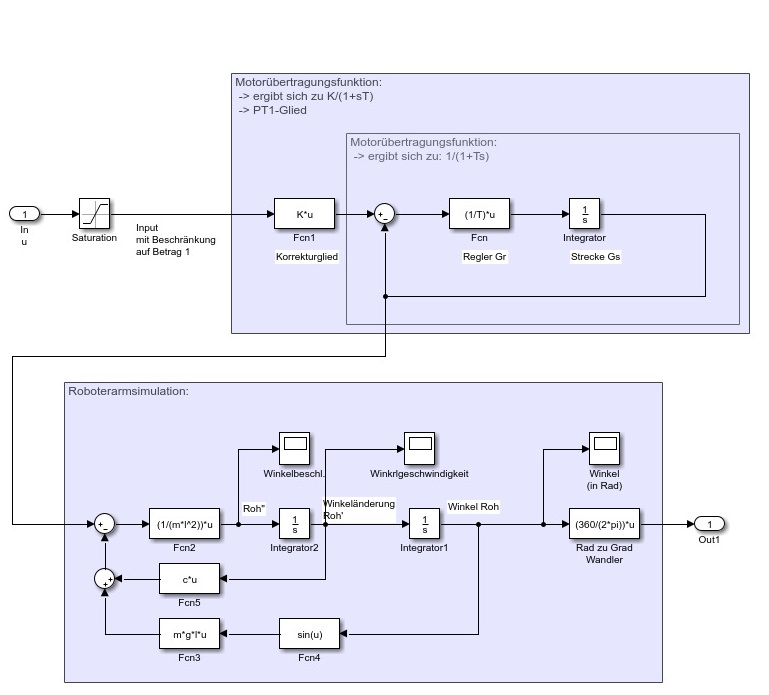
\includegraphics[width=0.7\textwidth]{Theoretischer Teil/SimulinkModell.jpeg}
	\caption{In Simulink gebautes Modell des Systems des Roboterarms}
	\label{img:grafik-dummy}
\end{figure}
%--------------------------------------------
%alte Grütze:
%Dieser bezeichnet das Aufstellen der Gleichungen aus den gegebenen Gleichungen. Die Gleichungen sind als Blockschaltbild gegeben. Diese werden jetzt %übersetzt in Mathlab Simulink.

%\begin{itemize}
%\item Startwerte
%Als Startwerte wurde gegeben:
%\begin{align}
%   	c &= 1 \\k &= 300  \\ T& = 0,1\\ g &= 9,81\, \frac{m}{s^2} \\l &= 1\, m\\m &= 7\, kg
%\end{align}
%\item Gegebenes Blockschaltbild:
%\begin{figure}[H]
%	\centering
%	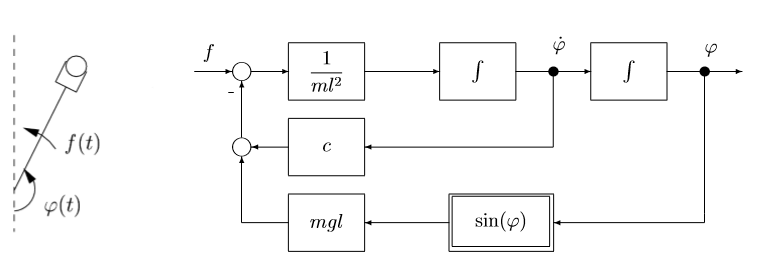
\includegraphics[width=0.6\textwidth]{Aufgabe9aMotorarm.png}
%	\caption{Motorarmmodell als Blockschaltbild}
%	\label{img:grafik-dummy}
%\end{figure}
%\begin{figure}[H]
%	\centering
%	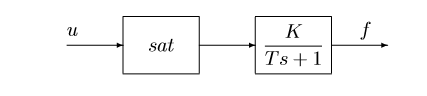
\includegraphics[width=0.6\textwidth]{Aufgabe9aStreckeMotor.png}
%	\caption{Modell des Motors als Blockschaltbild}
%	\label{img:grafik-dummy}
%\end{figure}
%\end{itemize}
%--------------------------------------------


\subsection{Wichtiger Hinweis:}
Für alle in diesem Bereich folgenden Auswertungen gibt folgende Farbkonvention
\begin{itemize}
\item Die rote Kurve entspricht dem Winkel $\varphi$
\item Die blaue Kurve entspricht dann der Winkelgeschwindigkeit $\dot \varphi$
\item Die grüne Kurve entspricht der Winkelbeschleunigung  $ \ddot \varphi$
\end{itemize}
%Version von Jonas und Christian vom 24.07.2019 am 13.08.2019 von Jonas überarbeitet



\subsection{Aufgabe 9.3.b Simulation ohne Eingangssignal mit Startwert}
Das System wird gemäß den Vorgaben simuliert und die Zustandsgrößen werden über einen Zeitverlauf dargestellt. Dabei entstehen das folgende Diagramm:

\begin{figure}[H]
	\centering
	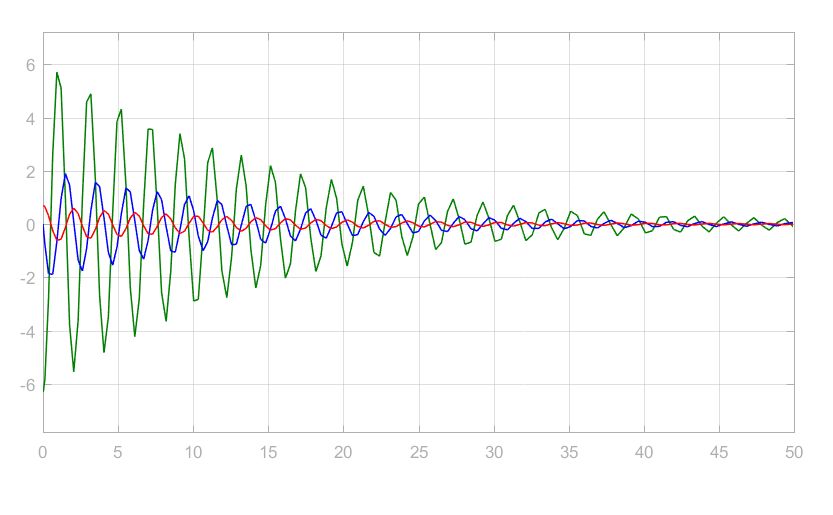
\includegraphics[width=1\textwidth]{9b}
	\caption{Darstellung des Winkels für eine anfängliche Auslenkung von 40 Grad. }
	\label{img:grafik-dummy}
\end{figure}

Aus dem obenstehenden Diagramm geht hervor, dass das System ein stabiles System darstellt, solange keine Stellgröße eingeprägt wird. Für gewöhlich kann das System eine Ruhelage bei 0\,$^\circ$ annehmen, wenn vorher keine Auslenkung vorgenommen wurde. Hier geht die Auslenkung auf keinen stationären Endwert, da die Expotentialfunktion zur Beschreibung der Dämpfung niemals null wird. In einem Realen System wird hier aber wahrscheinlich ein Stillstand nach beliebig langer Wartezeit eintreten, wenn der Roboterarm die Haftreibung nicht mehr Überwinden kann und die Bewegung im Aperiodischen Grenzfall endet.
\newpage
\subsection{Aufgabe c)}

%Version von Jonas und Christian vom 24.07.2019 am 13.08.2019 von Jonas überarbeitet



\subsection{Aufgabe 9.3.c  Simulation mit Eingangssignal ohne Startwert}
Es soll eine Simulation mit den folgenden Vorgaben durchgeführt werden: 
>>>>>>> Jonas
\begin{align}
\varphi  (0) &= 0 \\
\dot \varphi (0) &= 0 \\
u(t)  &= \binom{0\,\,\,\,\,\,\,\,\, für\,\, t<1}{0.17\,\, für\,\, t \geq 1}
\end{align}
%\varphi (0) &= 0 
%f(0) &= 0 
%
%u(t) &= 0 für t<1\\
%	0.17 für t >= 1;

\begin{figure}[H]
	\centering
	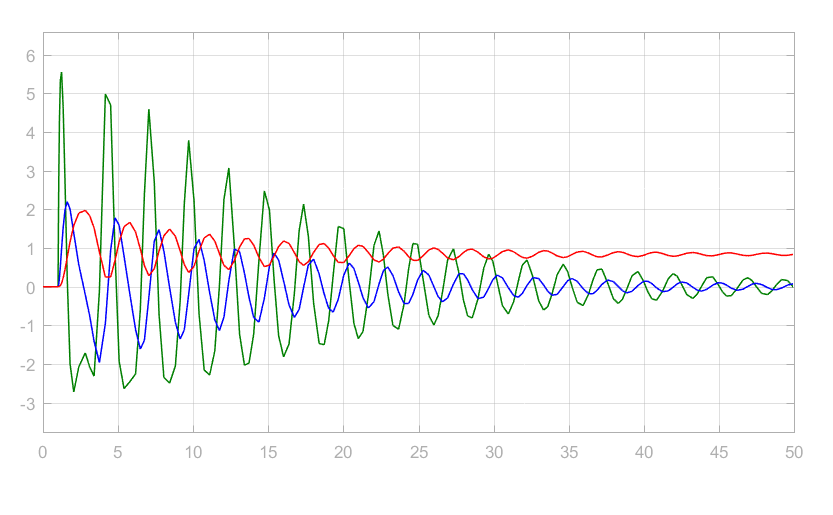
\includegraphics[width=0.8\textwidth]{9c}
	\caption{Darstellung des Winkels für eine anfängliche Auslenkung von 40 Grad. }
	\label{img:grafik-dummy}
\end{figure}

Das System befindet sich zunächst in Ruhelage zum Zeitpunkt \textit t = 1 wird ein Drehmoment vom Motor aufgebaut,
das den Roboterarm nach Durchlaufen eines Einschwingvorgangs um die neue Ruhelage in eben diese auslenkt.
Diese neue Ruhelage hängt von dem Eingangsdrehmoment ab. Der Einschwingvorgang weist dabei ein ähnliches Verhalten wie der Einschwingvorgang von Aufgabe 9.3b auf.
%Das Simulinkmodell des Roboterarms wird für die entsprechende Schaltung verändert. Alle Veränderungen werden in dieser Grafik dokumentiert.
%Danach wird das Modell linearisiert und das dann entstehende Ergebnis wird festgehalten



\subsection{Aufgabe 9.3.d Simulation mit Eingangssignal mit Startwert}
gegeben sei:
\begin{align}
\varphi  (0) &= 0 \\
\dot \varphi (0) &= 0 \\
u(t)  &= \binom{0\,\,\,\,\,\,\,\,\, für\,\, t<1}{0.18\,\, für\,\, t \geq 1}
\end{align}

\begin{figure}[H]
	\centering
	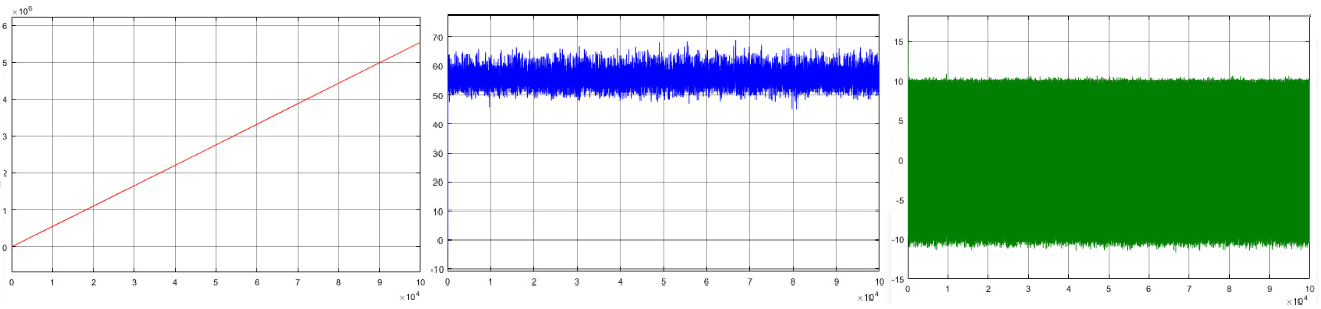
\includegraphics[width=1.2\textwidth]{Theoretischer Teil/Aufgabe9c.png}
	\caption{Darstellung des Winkels für eine anfängliche Auslenkung von 40 Grad. }
	\label{img:grafik-dummy}
\end{figure}

Anders als im Versuch 9.3.c befindet sich der Roboterarm nun zum Zeitpunkt \textit t = 0 nicht mehr in der Ruhelage bei einem Winkel von 0\,$^\circ$, 
sondern in einem Winkel von 40\,$^\circ$. Dies hat zur Folge, dass der Arm zunächst in der Zeit bis  \textit t = 1 sowie in der darauffolgenden Sättigungszeit des PT1-Gliedes das den Motor beschreibt, zurückschwingen kann.
Sobald das Drehmoment des Motors aufgebaut ist legt der Roboterarm an Geschwindigkeit zu und überschreitet dabei sogar die kritische 180\,$^\circ$
Marke, ab der der Arm nicht mehr zurückschwingt, sondern einen Überschlag vollführt und weiter an Geschwindigkeit gewinnt.
Da es sich bei dem betrachtetet Roboterarm um ein gedämpftes Model handelt, geht die Gewschwindigkeit in eine Sättigung über, bis diese um
einen konstanten Wert fluktuiert. 




\subsection{Aufgabe 9.3.e Überprüfung der These zur Positionsbeibehaltung}

Um zu überprüfen, ob der Motor bei einem Arm bei einem Eingangssignal von eine Ruhelage bei 40\,$^\circ$ zur Einstellung bringt. Wird dies in Mathlab mit folgendem Eingangssignal geprüft:

\begin{align}
   u_0 = \frac{m*g*l* sin( \varphi (0))}{300} = 0,1471
\end{align}
Dies entspricht einem Drehmoment von 44,1402 \textit N\textit m. Dieses Drehmoment wird im Modell als konstante Eingangsgröße augegebenen. Der resultierende Winkel wird dann in Grad angegeben und sollte entsprechend der Erwartung einen Winkel von 40\,$^\circ$ entsprechen.

\begin{figure}[H]
	\centering
	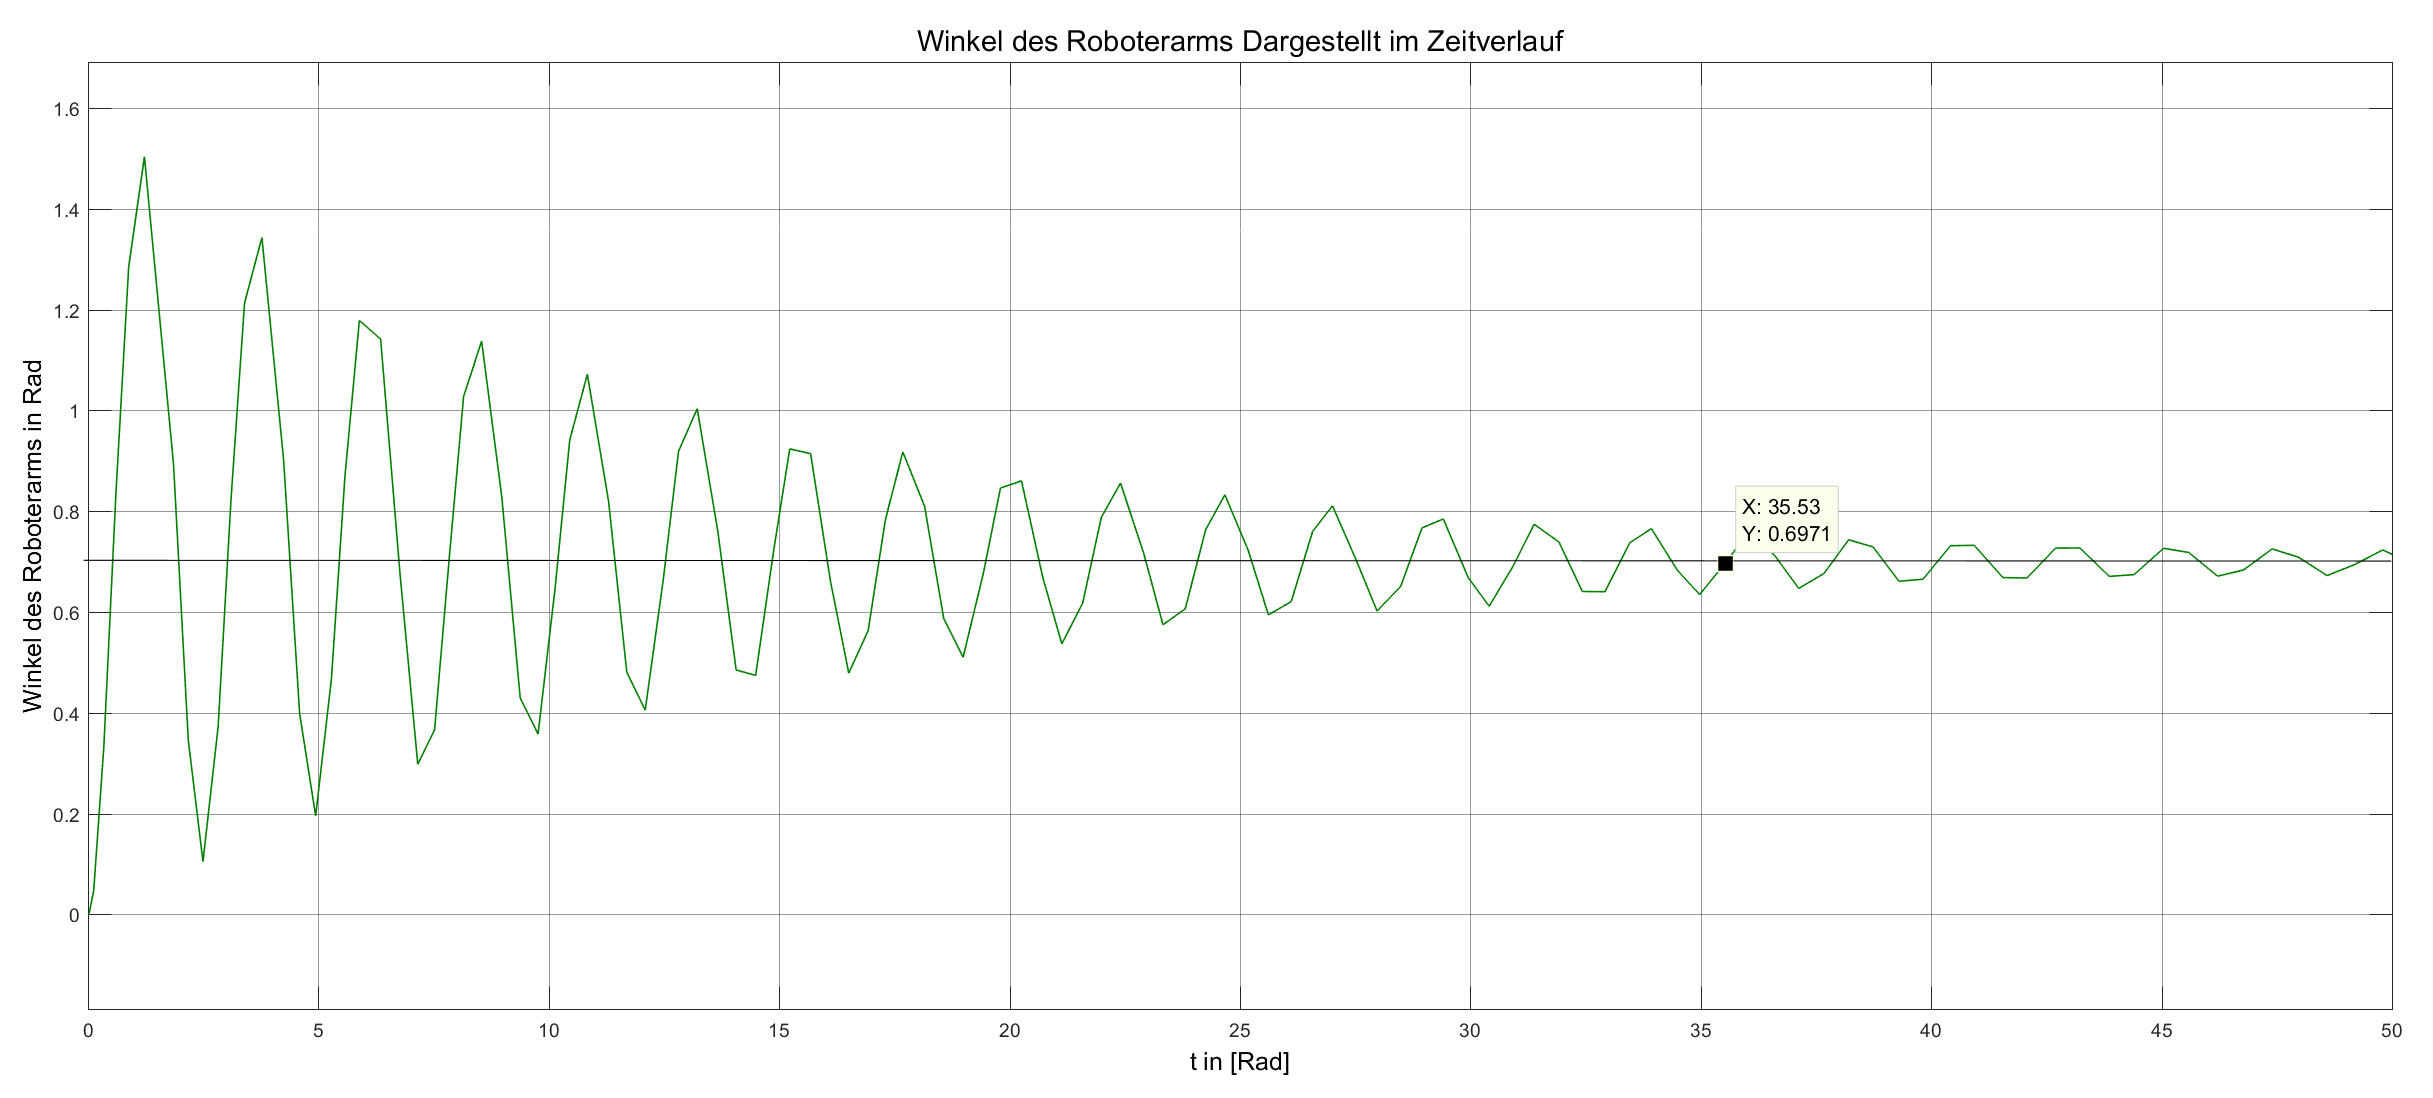
\includegraphics[width=1.2\textwidth]{Aufgabe9e}
	\caption{Darstelung des Winkelgraphen bei einem gegebenen Drehmoment}
	\label{img:grafik-dummy}
\end{figure}

An dem Diagramm ist explizit zu sehen, dass es sich bei der Auslenkung durch das Drehmoment u \textsubscript{0} einstellt. Diese Auslenkung entspricht im Mitte. einem Wert von 0,6971 Rad. Daraus ergibt sich eine neue Auslenkung von 40\,$^\circ$. Damit wird die Angabe aus dem Aufgabenscript bestätigt.




\subsection{Aufgabe 9.3.f Linearisierung des Modells}

Bei der Linearisirung durch Softwarenutzung von Mathlab ergibt sich folgendes Ergebnis für Winkel im Bogenmaß:

\begin{align}
   G_s = \frac{428.6}{(s^3 + 10.14*s^2 + 8.944*s + 75.15)} 
\end{align}

Die Abweichung zur Musterlösung in der dritten Nachkommastelle des Zählers lässt sich dabei durch einen veränderten Rundungsalgorithmus im Programm begründen. 
Die Ergebnisse stimmen also überein wodurch G\textsubscript{s} von nun an unsere Funktion der Strecke beschreibt.




\subsection{Aufgabe 9.3.g Reglerentwurf zur Stabilisierung}

Um einen Regler zu finden, der die Stabilitätskriterien einhält stellen wir zunächst die orginale Wurzelortskurve dar.

\begin{figure}[H]
	\centering
	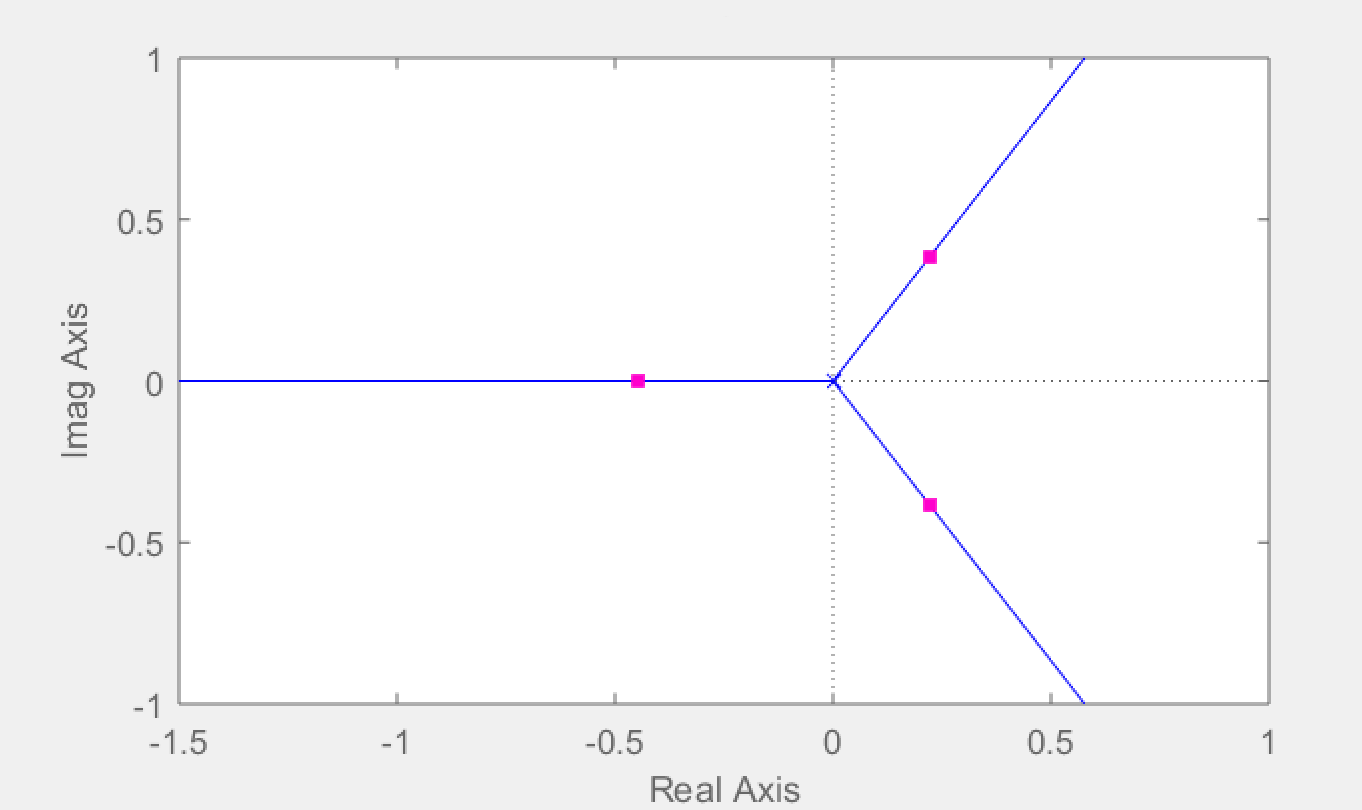
\includegraphics[width=0.8\textwidth]{WOZ9f}
	\caption{Wurzelortskurve des Systems G\textsubscript{s}}
	\label{img:grafik-dummy}
\end{figure}

In der Wurzelortskurve kann man direkt sehen, dass zwei Nullstellen in Richtung der zwei Nullstellen im positiven Bereich einen guten Regler darstellen würden. Diese müssen dabei nicht die die Polstellen kompensieren, sondern lediglich im Imaginären Anteil des Wurzel Ortskurve liegen um dort den die Zerphilien Anteile der Wurzelortskurve anzuziehen.
Es entsteht folgende Ausgabe:

\begin{figure}[H]
	\centering
	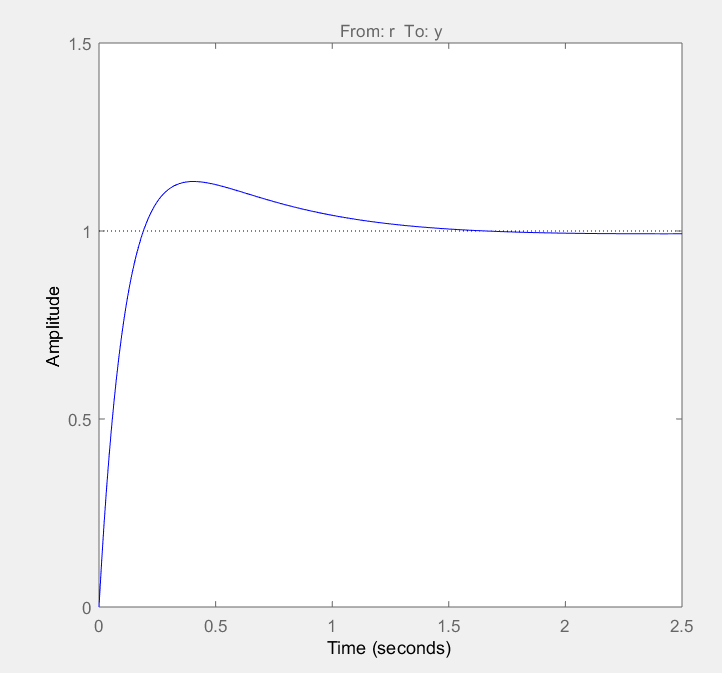
\includegraphics[width=0.6\textwidth]{WOZ9f2}
	\caption{Anzeige des Ausgangswertes}
	\label{img:grafik-dummy}
\end{figure}

Die sich damit realisierende Ausgabe wurde von dieser Wurzelortskurve erzeugt.
\begin{figure}[H]
	\centering
	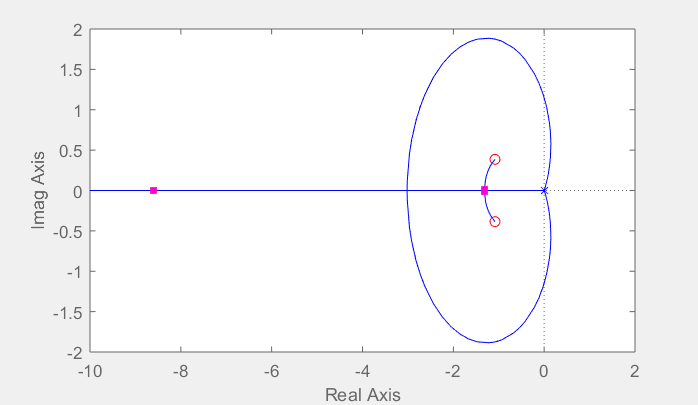
\includegraphics[width=0.8\textwidth]{WOZ9f3}
	\caption{Wurzelortskurve des Systems G\textsubscript{s} mit der Anpassung zweier Nullstellen}
	\label{img:grafik-dummy}
\end{figure}

<<<<<<< HEAD
Man sieht deutlich, dass es hier eine Stabilisierung der Funktion ergibt. Es ist natürlich keine unbegrenzte Stabilität von dem System zu erwarten. Der K-Wert sollte dabei so gewählt werden, dass die realen Pole alle im Linken teil der Kurve liegen sollten. Das wiederum hat dann die Folge, dass sich der K-Wert in einem gewissen Rahmen einstellen lassen können muss.
=======
\subsection{Aufgabe 9.3.h}
%missing input
>>>>>>> Jonas

%Präsensversuche
%----------------------------------------------------------------------------------------------------------------------------------------------------------------------------------------------------------------
\section{Versuch Antrieb}
\subsection{a)}	Die Sprungantwort des Systems soll ohne Filter ermittelt werden. Dabei zeigt sich jedoch das die Sprungantwort stark um den Wert von 300 fluktuiert.
	Nun soll die Sprungantwort mit eingeschaltetem Filter aufgenommen werden. Daraus wurde die Übertragungsfunktion durch ein PT1 Glied angenähert. Das Überschwingen wurde vernachlässigt. Die bestimmte Näherung lautet: 
\begin{align}
   G(s)_{PT1}=\frac{1275}{1+9,17s}
\end{align}
\subsection{c)}	Auf Basis der angenäherten Übertragungsfunktion kann nun ein Simulink Modell erstellt werden. Auf dies kann ein Regler ausgelegt werden und am realem Versuchsaufbau getestet werden.
\subsection{d)}	Die Vorgabe für den Regler soll eine t \textsubscript{5\%} Zeit von 0,3 Sekunden sein. Mithilfe einer Faustformel kann nun der Der Realteil des Poles bestimmt werden. Es ergibt sich dafür ein Realteil von -10 für den Pol des Geschlossenen Regelkreises des P Reglers. Der Geschlossene Regelkreis weist folgende Form auf:
\begin{align}
   G(s)_{PT1-geschlossen}=\frac{1275K_p}{1275K_p+9,17s}
\end{align}
%nun werden daraus die Pole in Abhängigkeit des Faktors K_p bestimmt. Daraus folgt das der Wert für K \textsubscript{p}=0,0711 betragen muss. 
\subsection{e)}	Der P-Regler wird nun am Simulink Modell getestet. Als Stationärer Endwert wird 1 angestrebt. Um diesen Zu erreichen wird eine Vorsteuerung mit dem Verstärkungsfaktor K \textsubscript{vor}= $ \frac{1600}{1581,5} $ die benötigte Stellgröße liegt über 5Volt aber im realistischen Bereich, dennoch liegt diese über 0,3 Sekunden lang an, sodass hier Handlungsbedarf besteht wenn das Reale System einen Error Code ausgibt.
\subsection{f)}	Der P-Regler wird mit Vorsteuerung an der realen Maschine getestet. Es fällt auf das die Maschine trotz eines überschreitens der kritischen Überspannungszeit in der Simulation korrekt arbeitet. Hier sind die Modellabweichungen so groß, dass wir die kritische Spannung weniger als 0,3 Sekunden  lang halten. Es lässt sich durch die nur näherungsweise zutreffende Streckenübertragungsfunktion in form eines PT1 Gliedes erklären. Das System ist nur für den einen Sollwert von 1600 Grad/sec stationär genau. Umso mehr die Sollwertgröße von 1600 Grad/sec abweicht desto Größer wird die Abweichung des Stationären Endwertes. Dies fällt erst bei weniger als 800 Grad/sec deutlich auf und ist bei 400 Grad/sec gut zu erkennen.
\subsection{g)}	Um Stationäre Genauigkeit für alle Sollwerte zu erreichen wird dem Regler ein I-Anteil hinzugefügt. Der PI-Regler wird über das SISO Tool ausgelegt. Aus den Anforderungen t \textsubscript{5\%}=0,4s und kein Überschwingen woraus sich ergibt das die Pole rein reell sein müssen ergibt sich für den schnellst möglichen Regler die Übertragungsfunktion
\begin{align}
   G(s)_{PI}=0,0074*\frac{1-7,1s}{s}
\end{align} 
ferner ist keine Vorsteuerung erforderlich, da der PI-Regler ohnehin eine stationäre Genauigkeit aufweist. 
6
	Statt dem PI-Regler soll nun eine Regelstruktur bestehend aus einem kaskadiertem P-Regler verwendet werden. Die Übertragungsfunktion 
\begin{align}
   G(s)_{p}=\frac{90653}{91,653+9,17s}
\end{align} 
	Die Übertragungsfunktion des Kaskadierten Reglers 
\begin{align}
G(s)_{ \dot{\theta}}=\frac{1}{s} = \frac{90,653}{91,653s+9,17s^2}
\end{align}
Mithilfe des SISO Tools kann ein P-Regler ausgelegt werden der die t \textsubscript{5\%} Zeit minimiert ohne dabei überzuschwingen. 
	Als Verstärkungsfaktor des P-Reglers wurde 2,5262 ermittelt.
	Die im bestimmte Kaskadenregelung soll nun in Simulink getestet werden. Als Sollwert wird dabei 90 Grad angenommen. Die dabei Benötigte Stellgröße liegt in einem realistischen Bereich und ist der Simulation nach zu Urteilen keine Gefahr für das reale System, da sie nicht länger als 0,3 Sekunden über einem Wert von 5 Volt liegt.\\
	Der zuvor in Simulink überprüfte Regler wird in das Reale System eingebaut und als Sollwert werden 90 Grad angelegt. Der Regler im echtem System bietet im Gegensatz zur Simulation keine Stationäre Genauigkeit. Dies liegt daran, dass das Modell keine Reibung berücksichtigt.
	Als Sollwert werden 10000 Grad angelegt.
%Ist Sollwert richtig?
 Allerdings ist dies ohne weiteres nicht möglich da das reale System einen Error Code ausgibt. 
Dies liegt an mehreren Problemen.
	Zuerst muss das Problem der Überspannung gelöst werden. Dies kann dadurch geschehen, dass ein Sättigungsblock in den Regelkreis eingebaut wird, sodass der Motor mit Maximal 5 Volt versorgt wird. Als nächstes muss die zu große Winkelgeschwindigkeit verringert werden. Dazu wird wieder ein Sättigungsblock eingebaut, weher die Winkelgeschwindigkeit auf Maximal 2000 Grad/sec wachsen lässt. Sind diese Probleme behoben kann der Motor in diesem Versuch einwandfrei benutzt werden. 
\subsection{Verbesserte Positionsregelung}
\subsubsection{Berechnen der Kaskadenregelung und der Führungsübertragungsfunktion}
Die Faustformel aus der Vorlesung schreibt folgende berechnung der Führungsübertragungsfunktion dar:
\begin{align}
   m=\frac{Im(\lambda)}{Re(\lambda)}
\end{align} 
Es soll der dominante Pol unter diesem hinblick untersucht werden. Dabei wird folgendes Ergebnis erziehlt:
\begin{itemize}
\item Berechnen der Pole der Streckenübertragungsfunktion und das prozentuale Überschwingen:
\begin{align}
G_{w} = \frac{186,0496}{(s+13,46) * (s-13,46)}
\end{align} 
Daraus ergeben sich folgende Polstellen:
\begin{align}
 x_1 = 23.4600 ,\,\,\
 x_2 =-10.0000 -13.4600i
\end{align}

\item \subsubsection{Bestimmen der Verstärkung des P-Reglers} Bestimmen der P-Regelkoeffizienten dieser Anordnung kann folgend vorgenommen werden:
Bei der Anordnung können die kaskadierten Werte der P-Regler K\textsubscript{P} und K\textsubscript{I} 

Allgemein gilt für die Formel:
\begin{align}
G_{w} = \frac{\frac{K_P * K_s*K_D}{T}}{s^2+(\frac{K_D*K_P}{T}+\frac{1}{T})*s+\frac{K_P*K_I*K_S}{T}}
\end{align} 
\begin{align}
G_{w} = \frac{186,0496}{(s+13,46) * (s-13,46)}
\end{align} 
Aus der oben genanten Gleichung kann also gefolgert werden:
\begin{align}
\frac{K_P * K_s*K_I}{T} =186,0496
\end{align}
Wir können also K\textsubscript{R} bestimmen als:
\begin{align}
K_P * K_I = K = 0,04377637647
\end{align}
% m_{\Delta}=\frac{Im(\lambda)}{Re(\lambda)} ,\
\item \subsubsection{Simulieren des Regler und Überprüfung auf die Vorgaben}
\begin{figure}[H]
	\centering
	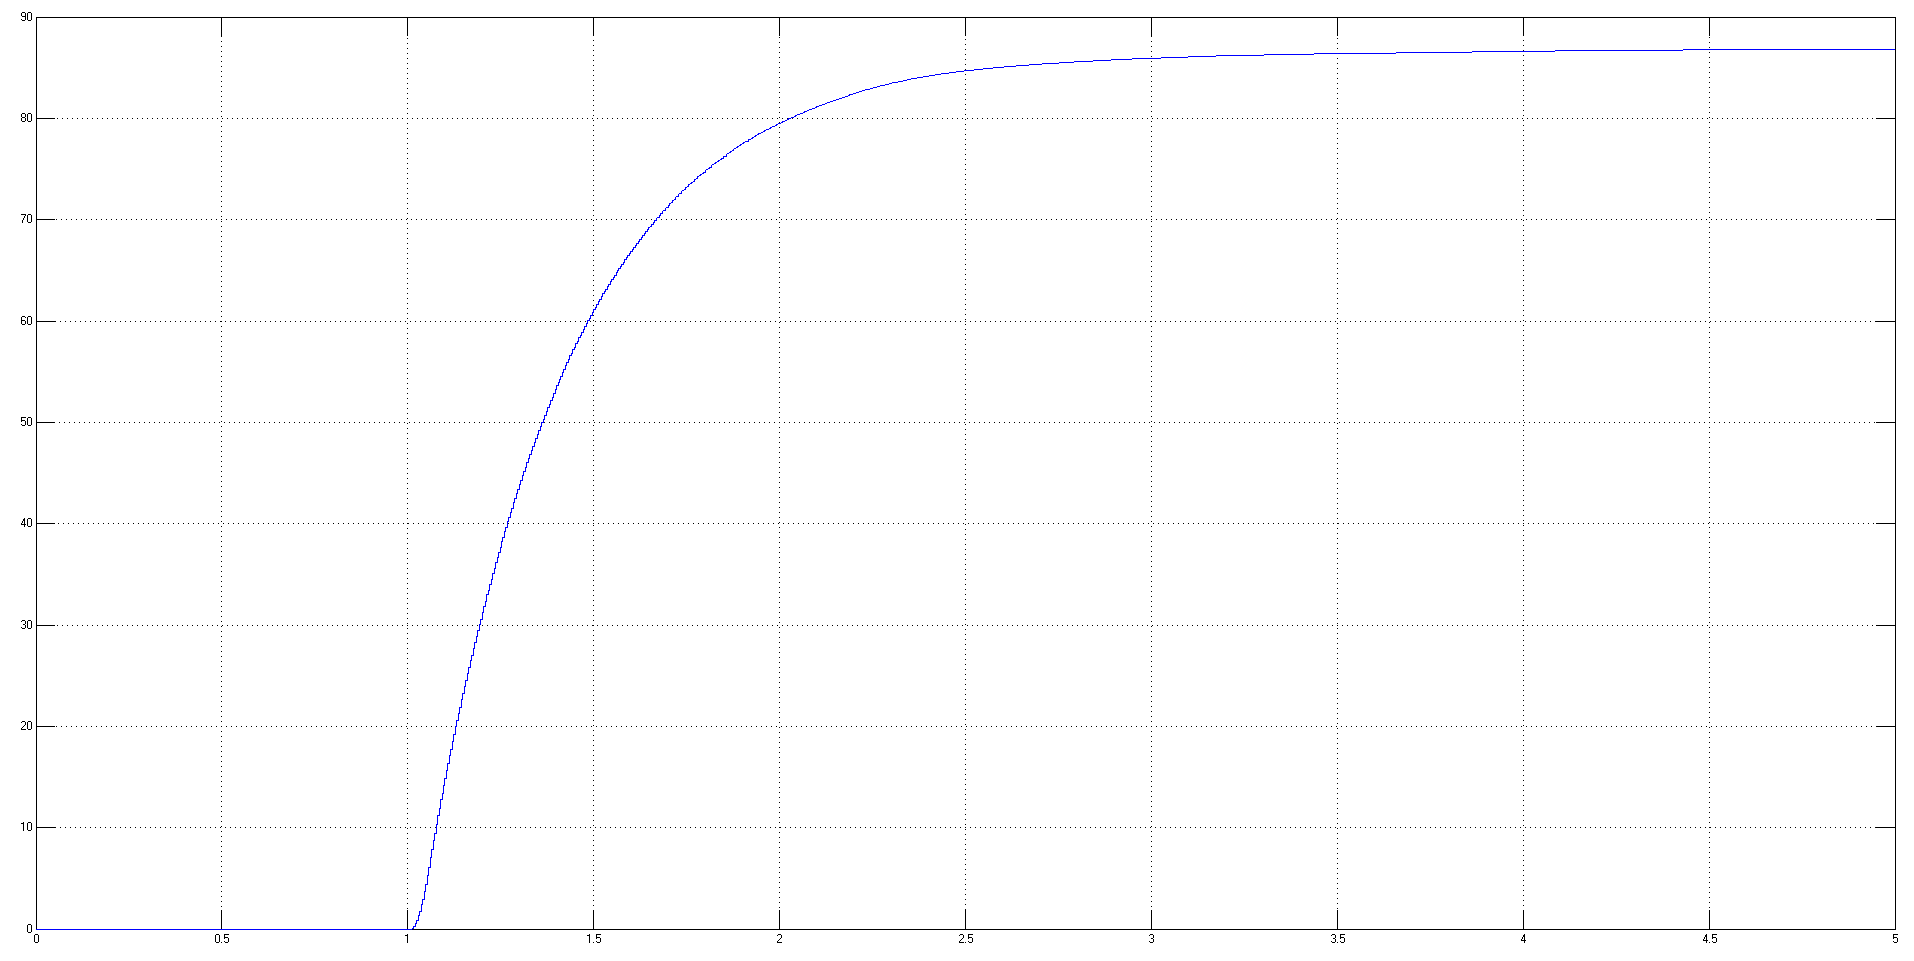
\includegraphics[width=1.1\textwidth]{Drehzahl6e3neu.png}
	\caption{Simulation der berechneten Regelgrößen und der Berechneten K-Werte bei der Führungsgröße 90 $^\circ$.}
	\label{img:grafik-dummy}
\end{figure}
Anhand der Führungsgröße bleibt zu sehen, dass nun angepasst Verhalten von  $\Delta$ m und t\textsubscript{5\%}.
Beim Ablesen der Werte aus dem Diagramm können folgende Werte Festgehalten werden:
\begin{align}
\Delta m = 0
\end{align}
Dies könnte ebenfalls daraus gefolgdert werden, dass es sich um ein PT-1-Glied handelt und diese in keinem Fall ein Überschwingen erzeugen.
\begin{align}
t\textsubscript{5\%} = 3s
\end{align}
Die t\textsubscript{5\%} Zeit liegt mit 3 Sekunden im erwarteten Rahmen.
\end{itemize}

\subsubsection{Implementation und versuch an der Maschine im Praktikum}
Der Test im realen System zeigt, dass das System sich real nicht, wie ein PT-1-Glied verhält. Dies ist vorallem mit den sehr hohen Reibungskoeffizienten am Versuchsaufbau zu erklären. Daraus ergibt sich folgendes Diagramm der Drehung um 90 $^\circ$.
\begin{figure}[H]
	\centering
	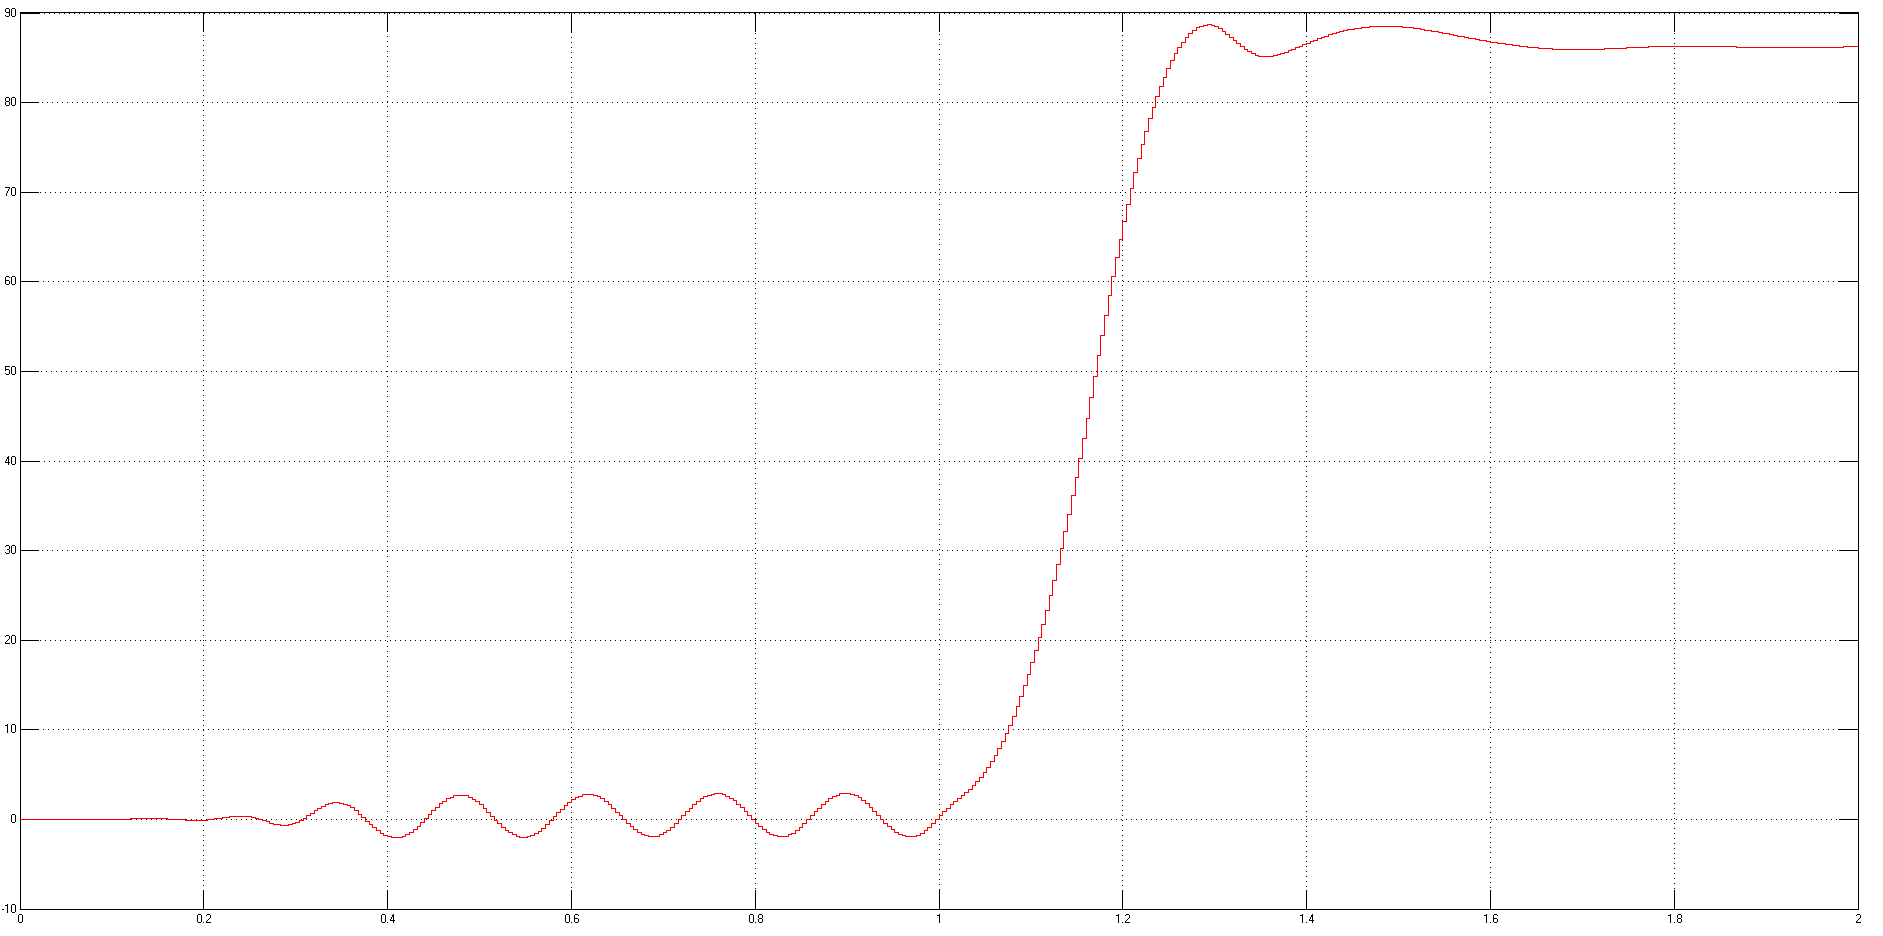
\includegraphics[width=1.2\textwidth]{Drehzahl57B.png}
	\caption{Realer Messwert des Systems bei einer geregelten Drehung um 90 $^\circ$}
	\label{img:grafik-dummy}
\end{figure}
Man könnte im Nachgang diesen Versuch mit etwas Öl auf den Lagern wiederholen um verbesserte Ergebnisse zu erzielen, ein Überschwingen ist ebenfalls nicht eingetreten allerdings hat der Verlauf des realen System nicht die erwarteten gemeinsamkeinten mit einer PT-1-Strecke.
\newpage



%--------------------------------------------------------------------------------------------------------------------------------------------------------------------------------
\section{Versuch Schwebekörper}
%--------------------------------------------------------------------------------------------------------------------------------------------------------------------------------


\subsection{Einstieg in den Praktikumsversuch}
Zu Begin dieses Praktikumsversuchs gilt es, sich Mittels Joystick mit der Anlage vertraut zu machen. Dabei fällt schnell auf, dass die Voreinstellungen der Scope-Blöcke noch nicht sinnvoll gewählt worden sind. Um die graphische Ausgabe physikalisch sinn-voll darzustellen, müssen die Skalierung der Eingangsgröße sowie eine y-Achsenver-schiebung wie folgt vorgenommen werden:

\begin{enumerate}
\item Die Stellgröße des Systems muss auf Grund des im Experiment verbauten Leistungsteil für den Lüfter mit dem Faktor 1,2 skaliert werden.
\item Die Regelgröße muss zunächst negiert werden, um einen positiven Ausschlag zu erzeugen. Anschließen wird der Offset eliminiert und der Maximale Ausschlag des Systems richtig skaliert, sodass sich eine Anpassung von


\begin{align}
   G_{(s)}=\frac{-Tatsächliche Maximale Höhe*(Eingang-Offset)}{Vorläufige Maximale Höhe}
\end{align}
\begin{align}
= -18,34*(u-6)
\end{align}
\end{enumerate}
ergibt.


\subsection{Mathematisches Modell erstellen}
Ein mathematisches Modell lässt sich dank des zur Verfügung stehenden Mathlab-Skripts \textit {grafident.m} durch Ausführen des Skriptes leicht erstellen. Das Skript gibt einen grafischen Verlauf der Sprungantwort und die wichtigsten Kenngrößen aus.

\begin{figure}[H]
	\centering
	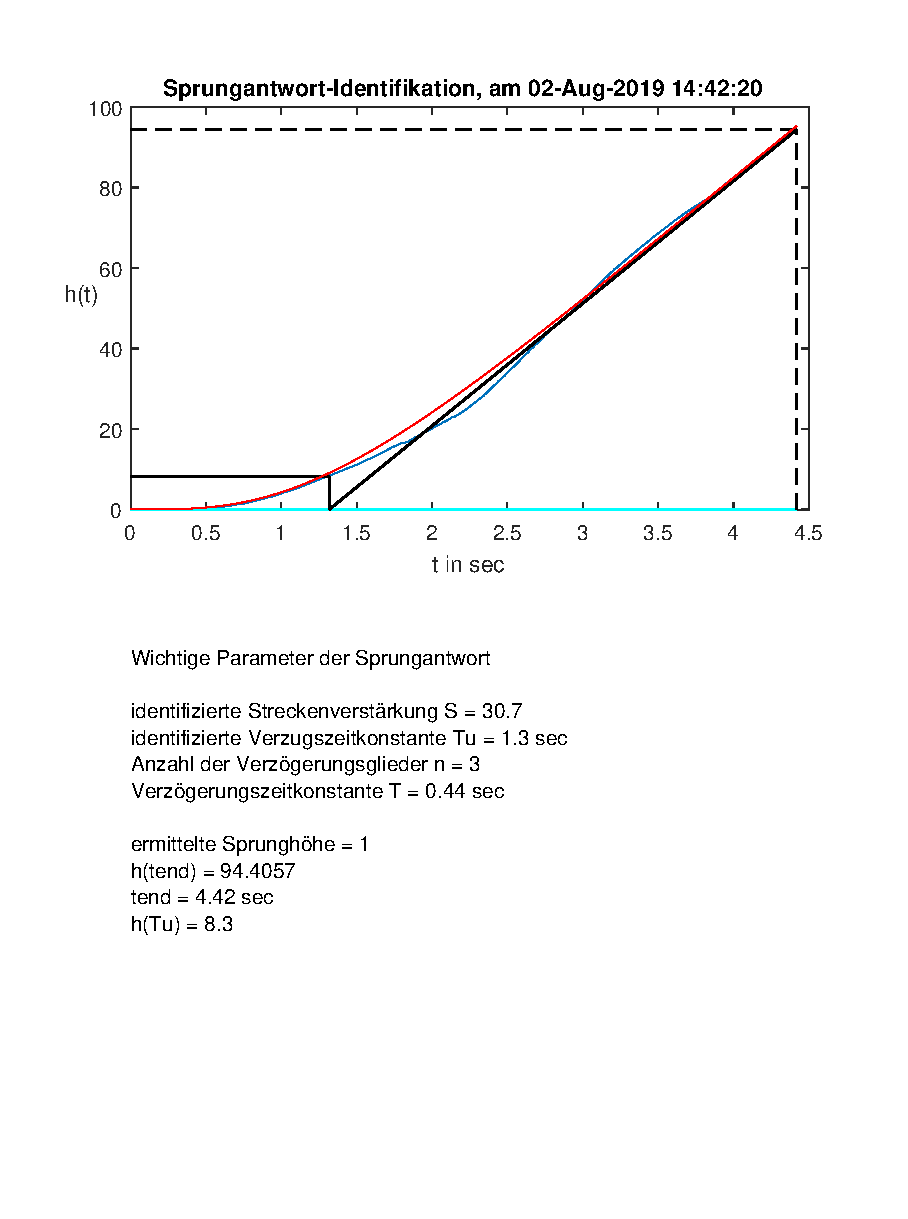
\includegraphics[width=0.6\textwidth]{SchwMod}
	\caption{Anzeige des Ausgangswertes}
	\label{img:grafik-dummy}
\end{figure}



\subsection{Regelungsziele definieren}
Generell sind natürlich minimale Einschwingzeit und möglichst geringes Überschwingen erwünscht. Häufig lassen sich jedoch diese beiden Parameter nicht gentrennt von einander optimieren. Unser Regelziel ist an dieser Stelle eine Einschwingzeit von
\begin{align}
t\textsubscript{5\%} = 3
\end{align}
 und ein Überschwingen, dass nicht den Versuchsaufbau verletzt.



\subsection {Entwurf eines einfachen Reglers}
Es soll nun mithilfe des jetzigen Kenntnisstands ein möglichst einfacher Regler entworfen werden, der den Schwebekörper auf einer Wunschposition halten kann. Hier erfüllt ein P-Regler mit einer Verstärkung von \textit K = 0,012954 zunächst noch die vorgegebenen Vorraussetzungen.

%Hier wird bei Jonas ein Bild angezeigt, dass gar nicht hier her gehört

\subsection{Test des einfachen Reglers am System}
Testet man nun das Modell am realen System, treten deutliche Abweichungen auf. Es benötigt wesentlich länger um die vorgegebene Höhe zu erreichen. Hat es die Wunschhöhe erreicht, kommt es vor, dass der Schwebekörper nochmal aus der Position ausbricht und anschließend neu eingeregelt werden muss. Das System scheint auf Störungen zu reagieren, wie zum Beispiel das Berühren der Röhrenwand, die im Modell nicht berücksichtigt wurden.


\newpage
%--------------------------------------------------------------------------------------------------------------------------------------------------------------------------------
\section{Versuch Kran}
%---------------------------------------------------------------------------------------------------------------------------------------------------------------------------------
% subsection sollte rausfliegen
%\subsection{Vorbereitungsaufgaben}
%Welcome to Jonas part3
\subsection{Regelung der Wagenposition y\textsubscript{w}}


\subsubsection {Arbeitsposition einnehmen}
Der Kran ist in die zukünftige Arbeitsposition zu bewegen, das bedeutet er soll sich auf der mittleren x\textsubscript{w}-Position sowie auf der mittleren R-Position (Höhenposition) befinden. Diese beiden Parameter sowie die dazugehörigen Stellgrößen bleiben für den Rest des Versuchs unverändert, während in der y\textsubscript{w}-Richtung gearbeiten wird. 
Dafür gibt es prinzipiell verschiedene Möglichkeiten:

\begin{enumerate}
\item Man kann den Kran mit Hilfe der Bedienoberfläche (Aufruf mit Hilfe des commands \textit{cr}) „3DCrane“ ansteuern. Hier ist unter dem Begriff Tools der Button „Go To Center“ zu finden, der dafür sorgt, dass der Kran sich automatisch in die mittlere x\textsubscript{w}- sowie R-Position begibt.
\item In der Bedienoberfläche finden sich neben diversen Commandpresets auch das Tool „Manual Setup“ mit dem man die Parameter des Krans sowohl ablesen als auch manuell einstellen kann.
\end{enumerate}


\subsubsection {Messung der Haftreibung}

In Aufgabe 4.3.b gilt es, die Haftreibung des Kransystems zu bestimmen, da diese später eine direkte Auswirkung auf die Regelung haben wird. Dafür wird  zunächst sichergestellt, dass sich der Kran in Ruhe befindet und alle Stellgrößen gleich Null sind. Nun kann die Spannung die als „Y control“ Stellgröße benötigt wird, um den die Haftreibung des Wagens zu überwinden zunächst grob geraten werden und in einem zweiten Schritt genauer bestimmt werden. Es ergibt sich experimentell eine Spannung von:

\begin {align}
 u\textsubscript{y} = 0,059 
\end{align}


\subsubsection {Einfacher Proportionalregler}
In Aufgabenteil 4.3.c soll ein linearer Positionsregler herangezogen werden, der direkt proportional zur Abweichung der Position zur Wunschposition die Spannung \textit{ u\textsubscript{y}} bestimmt.
Nach der im Skript geforderten Vorgabe, soll die aus einer Positionsabweichung von 2\textit{cm} resultierende Stellspannung \textit{ u\textsubscript{y}} gerade noch so genügen, um die Haftreibung des Systems zu überwinden. (Dies bedeutet gleichzeitig, dass wir versuchen, den Wagen mind. auf 2\textit{cm} genau einzuregeln.) 
Durch Umstellen der gegebenen Formel 

\begin {align}
u\textsubscript{y}=R\textsubscript{y}*(\bar{y}\textsubscript{w}-y\textsubscript{w}) 
\end{align}

ergibt sich ein Verstärkungsfaktor von 

\begin {align}
Ry=2,95
\end{align}


\subsubsection {Maximale Auslenkung innerhalb der Sättigung}

Nun soll ermittelt werden, ab welchem Regelfehler das Stellsignal für 
\textit{R\textsubscript{y}} = 5 die Sättigung erreicht. 
Dies lässt sich mit der vorangestellten Formel durch Einsetzen lösen. 
Man erhält eine Abweichung von 20\textit{cm}, ab denen das System nicht stärker regelt.


\subsubsection {Implementierung des Reglers mit verschiedenen Parametern}

Im Folgenden werden drei verschiedene Implementierungen dieses Reglers betrachtet (und hinsichtlich der Positionsgenauigkeit, Geschwindigkeit und Pendeldauer begutachtet):\newline
Gegeben sind der Verstärkungsfaktor\textit{R\textsubscript{y}} und die Positionsabweichung von der Wunschposition

\begin{align}
\textit{R\textsubscript{y}} = 5 \bar{y}\textsubscript{w}-y\textsubscript{w} = 0,2 
\end{align}

%1.	Ry = 5		yquerw-yw = 0.2
%2.	Ry = 5		yquerw-yw = 1
%3.	Ry = 1,5	yquerw-yw = 1








\newpage
%end of Jonas part3
\subsection{ZusätzlicheRregelung des Winkels $\alpha$ }
Februar 2019 durchgeführt.
a)	Es handelt sich um ein um die Ruhelage linearisiertes Zeitinvariantes System. Dies im LTI Block implementiert wird. Die Rückkopplungen sind ebenfalls Linear weshalb die gesamte Regler Struktur Linear ist.
Das Linearisierte Modell kann in zwei Versionen in Mathlab bzw. Simulink implementiert werden:
1) Es kann über die Verschiedenen Beziehungen der einzelnen Zustandsgrößen und Eingangsgrößen ein Simulink Modell erstellt werden.
2) Die Linearisierten Gleichungen in Matrizen Form können direkt in Mathlab eingegeben werden, woraus Mathlab selbstständig ein LTI System realiesiert. 
Beide Varianten liefern das gleiche Ergebnis.
Wir benutzten den 1. Weg. 
%Zweigrafiken nebeneinander: Schema
%\begin{figure} 
%    \subfigure[Bezeichnung der linken Grafik]{\includegraphics[width=0.49\textwidth]{ordner/name1.jpg}} 
%    \subfigure[Bezeichnung der rechten Grafik]{\includegraphics[width=0.49\textwidth]{ordner/name2.jpg}} 
%\caption{Titel unterm gesamten Bild} 
%\end{figure}
\begin{figure}  %Darauf achten, dass diese Figur an der richtigen Stelle ist
    \subfigure[Simulink Modell ]{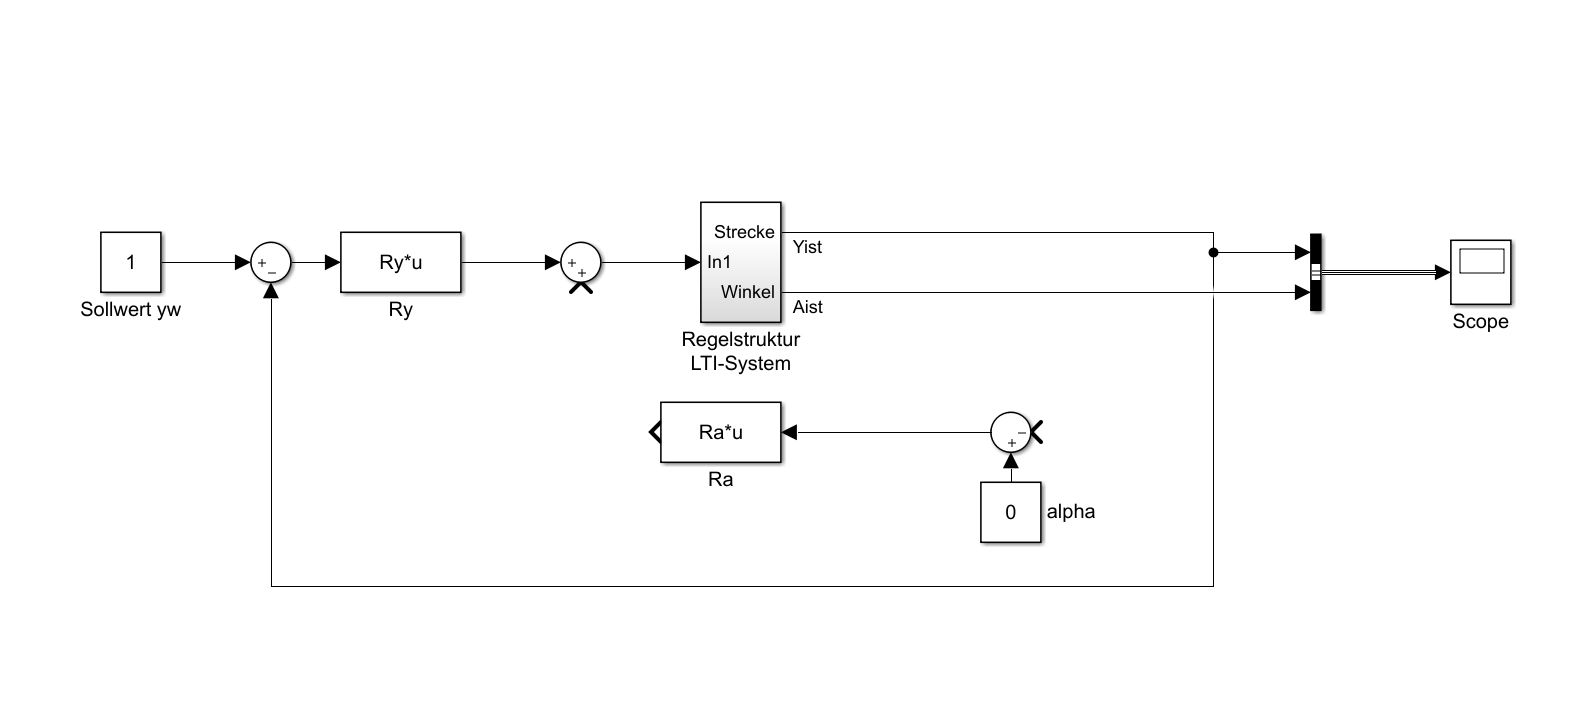
\includegraphics[width=0.6\textwidth]{Leon-PRT-Bilder/Simulink1}} 
    \subfigure[Simulink LTI Block]{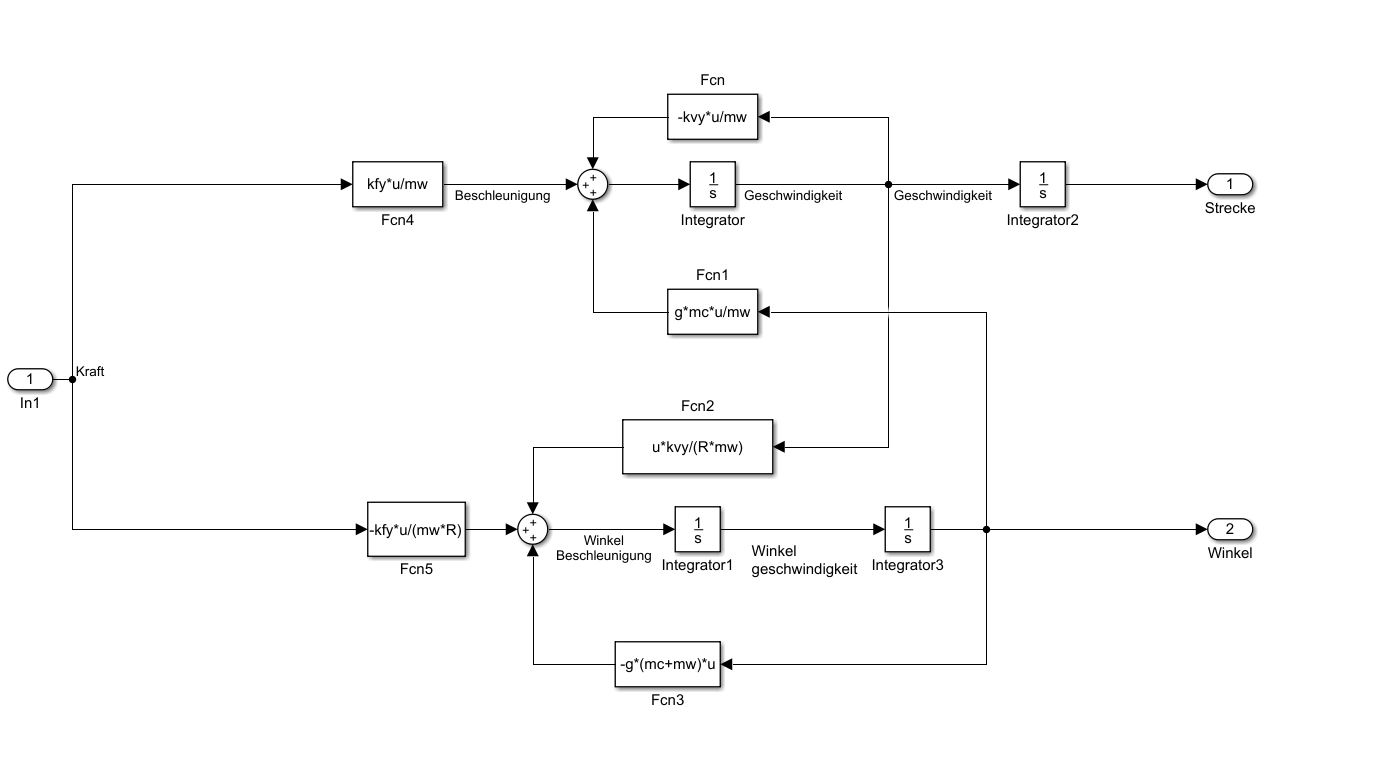
\includegraphics[width=0.42\textwidth]{Leon-PRT-Bilder/Simulink2}} 
\caption{Simulink Modell mit aufgetrennter Rückkoplung} 
\end{figure}
Aus dem Modell werden die Übertragungsfunktion und ihre Pole bestimmt.
\begin{align}
   G_{(s)}=\frac{-34,18s+0,04443}{s^3+48,51s^2+954,4}
\end{align}
%G_Strecke (S)=(-34,18s+0,04443)/(s^3+48,51s^2+954,4)
Diese Übertragungsfunktion besitzt folgende Pole:
\begin{align}
-48,3558 \notag \\
-0,0939+4,437i  \notag \\
-0,0939-4,437i \notag 
 \end{align} 
Davon entfallen folgende Pole auf die Last: 
\begin{align}
-0,0939+4,437i  \notag \\
-0,0939-4,437i  \notag 
\end{align}
Und dementsprechend entfällt auf den Kran der folgende Pol:
\begin{align}
-48,3558  \notag 
\end{align}
Die Last ist, im Gegensatz zum Wagen, schwingungsfähig, weshalb diese Pole einen imaginären Anteil aufweisen. Die Pole des Wagens werden hingegen rein reell modelliert. 
Daraus ergibt sich die über die Faustformel für das Einschwingen in das 5\% Band Folgender Ausdruck
\begin{align}
t_{(5\%)}=\frac{-3}{Re(s_D)}=33,3
\end{align}
%d)
 Als sinnvolle Einschwingzeit für das geregelte System wurde eine Einschwingzeit von  3,3 Sekunden gewählt, was einer Dekade weniger als die des ungeregelten Systems beträgt. Aus dieser Überlegung ergibt sich als gewünschter Überlegung über die obrige Faustformel ein Realteil des dominanten Poles der Last von -1. Über eine Bedingung für die Maximale Überschwingweite könnten nun die Imaginär Anteile bestimmt werden. (Hier nicht gegeben.) \\
%e)
Mithilfe des SISO Tools kann der Regler Parameter R \textsubscript{a}
über die Wurzelortskurve und die Sprungantwort bestimmt werden.
R \textsubscript{a} = - 2,6
%f)
Das System soll nun simuliert werden für die festgelegten Parameter
R \textsubscript{a} = 1
 y \textsubscript{w} = 1
% \begin{align}
%   R _a = 1
% \end{align}
% \begin{align}
 %  y_w &= 1
% \end{align}
Daraus ergibt sich das folgende Ergebnis: 
%MUss noch in eps format umgewandelt werden
%\begin{figure} 
 %   \subfigure[4.4b]{\includegraphics[width=0.49\textwidth]{Leon-PRT-Bilder/Fig44b}} 
%    \subfigure[XXXX]{\includegraphics[width=0.49\textwidth]{Leon-PRT-Bilder/Fig44b}} 
%\caption{XXXXXXXXXXXXXXX} 
%\end{figure}
(g+h) Der Regler soll nun am Realem System getestet werden
Der Regler dämpft die Schwingung deutlich besser als das ungeregelte System. Es liegt aber trotzdem weit weg von der Simulation bei der wir nach 3,3 Sekunden im 5\% Band liegen. Im Vergleich, dieser Zustand ist im realem System erst nach ca. 5,5 Sekunden erreicht. Dennoch liegt die Maximale Winkelauslenkung des Realem Systems unter der der Simulation. Das verlangsamte einschwingen kann durch die Sättigung des Motors erklärt werden, welcher nur bei Spannungen bis ?5Volt? die Regelung des Winkes einbeziehen kann. Das führt dazu, dass die Regelung erst später beginnt zu arbeiten und damit das System langsamer wird. Die Regelung arbeitet die Erste 2,5 Sekunden nicht und diese Braucht das reale System länger um die Ruhelage zu erreichen. Das Maximale Überschwingen ist geringer, da der Motor auch die Bewegung in y Richtung nicht beliebig Schnell durchführen kann sondern auch hier gesättigt ist. Außerdem wurde im Modell keine Gleitreibung berücksichtigt.

Antrieb 
5: Drehzahlregelung
	Die Sprungantwort des Systems soll ohne Filter ermittelt werden. Dabei zeigt sich jedoch das die Sprungantwort stark um den Wert von 300 fluktuiert.
 
	Nun soll die Sprungantwort mit eingeschaltetem Filter aufgenommen werden. Daraus wurde die Übertragungsfunktion durch ein PT1 Glied angenähert. Das Überschwingen wurde vernachlässigt. Die bestimmte Näherung lautet: 
\begin{align}
G(s)_{PT1}=1275/(1+9,17s)
 \end{align}
	Auf Basis der angenäherten Übertragungsfunktion kann nun ein Simulink Modell erstellt werden. Auf dies kann ein Regler ausgelegt werden und am realem Versuchsaufbau getestet werden.
	Die Vorgabe für den Regler soll eine t(5\%) Zeit von 0,3 Sekunden sein. Mithilfe einer Faustformel kann nun der Der Realteil des Poles bestimmt werden. Es ergibt sich dafür ein Realteil von -10 für den Pol des Geschlossenen Regelkreises des P Reglers. Der Geschlossene Regelkreis weist folgende Form auf: 
\begin{align}
G(s)_(geschl.)=(1275K_p)/(1275K_p+ 1+9,17s)
 \end{align}
 nun werden daraus die Pole in Abhängigkeit des Faktors Kp bestimmt. Daraus folgt das der Wert für 
\begin{align}
K_p=0,0711
 \end{align} 
betragen muss. 
	Der P-Regler wird nun am Simulink Modell getestet. Als Stationärer Endwert wird 1 angestrebt. Um diesen Zu erreichen wird eine Vorsteuerung mit dem Verstärkungsfaktor 
\begin{align}
K_vor=\frac{1600}{1581,5}
 \end{align} 
 die benötigte Stellgröße liegt über 5Volt aber im realistischen Bereich, dennoch liegt diese über 0,3 Sekunden lang an, sodass hier Handlungsbedarf besteht wenn das Reale System einen Error Code ausgibt.
	Der P-Regler wird mit Vorsteuerung an der realen Maschine getestet. Es fällt auf das die Maschine trotz eines überschreitens der kritischen Überspannungszeit in der Simulation korrekt arbeitet. Hier sind die Modellabweichungen so groß, dass wir die kritische Spannung weniger als 0,3 Sekunden  lang halten. Es lässt sich durch die nur näherungsweise zutreffende Streckenübertragungsfunktion in form eines PT1 Gliedes erklären. Das System ist nur für den einen Sollwert von 1600 Grad/sec stationär genau. Umso mehr die Sollwertgröße von 1600 Grad/sec abweicht desto Größer wird die Abweichung des Stationären Endwertes. Dies fällt erst bei weniger als 800 Grad/sec deutlich auf und ist bei 400 Grad/sec gut zu erkennen.
	Um Stationäre Genauigkeit für alle Sollwerte zu erreichen wird dem Regler ein I-Anteil hinzugefügt. Der PI-Regler wird über das SISO Tool ausgelegt. Aus den Anforderungen t(5\%)=0,4s und kein Überschwingen woraus sich ergibt das die Pole rein reell sein müssen ergibt sich für den schnellst möglichen Regler die Übertragungsfunktion 
$G(s)_PI=0,0074*(1-7,1s)/s$ ferner ist keine Vorsteuerung erforderlich, da der PI-Regler ohnehin eine stationäre Genauigkeit aufweist. 

\subsection{Digitale PD-Regelung von  y\textsubscript{w} und $\alpha$}
\subsubsection{Einfluss der Abtastzeit}

In diesem Versuch wird der Einfluss der Abtastzeit auf das Ergebnis der Regelung genommen. Da wir die Regelfunktion des PD-Regler diskretisiert haben und danach sich das Ergebnis im k Bereich befindet, muss dieses Ergebnis dann noch in die Bildebene Z gebracht werden. 
%TODO Deltas aus dem Text entfernen!
\begin{align}
   G(s)_R = K_P + K_D s = K_P *s + K_D *·(1 + s *T_D)  \\
   y_k= K_P * k+ \frac{K_D}{T_D} *( k - 1 )  \\
   G(z)_R = K_p * z + \frac{K_D}{T_D*T} *\frac{z-1}{z}
\end{align}
Was dabei einkalkuliert wurde, ist, dass T direkt die Abtastzeit des Reglers Berücksichtigt und daraus sich der Regelkreis beeinflussen lässt.
\begin{enumerate}
\item Die Abstastzeit wird auf t = festgelegt.
\begin{figure}[H]
	\centering
	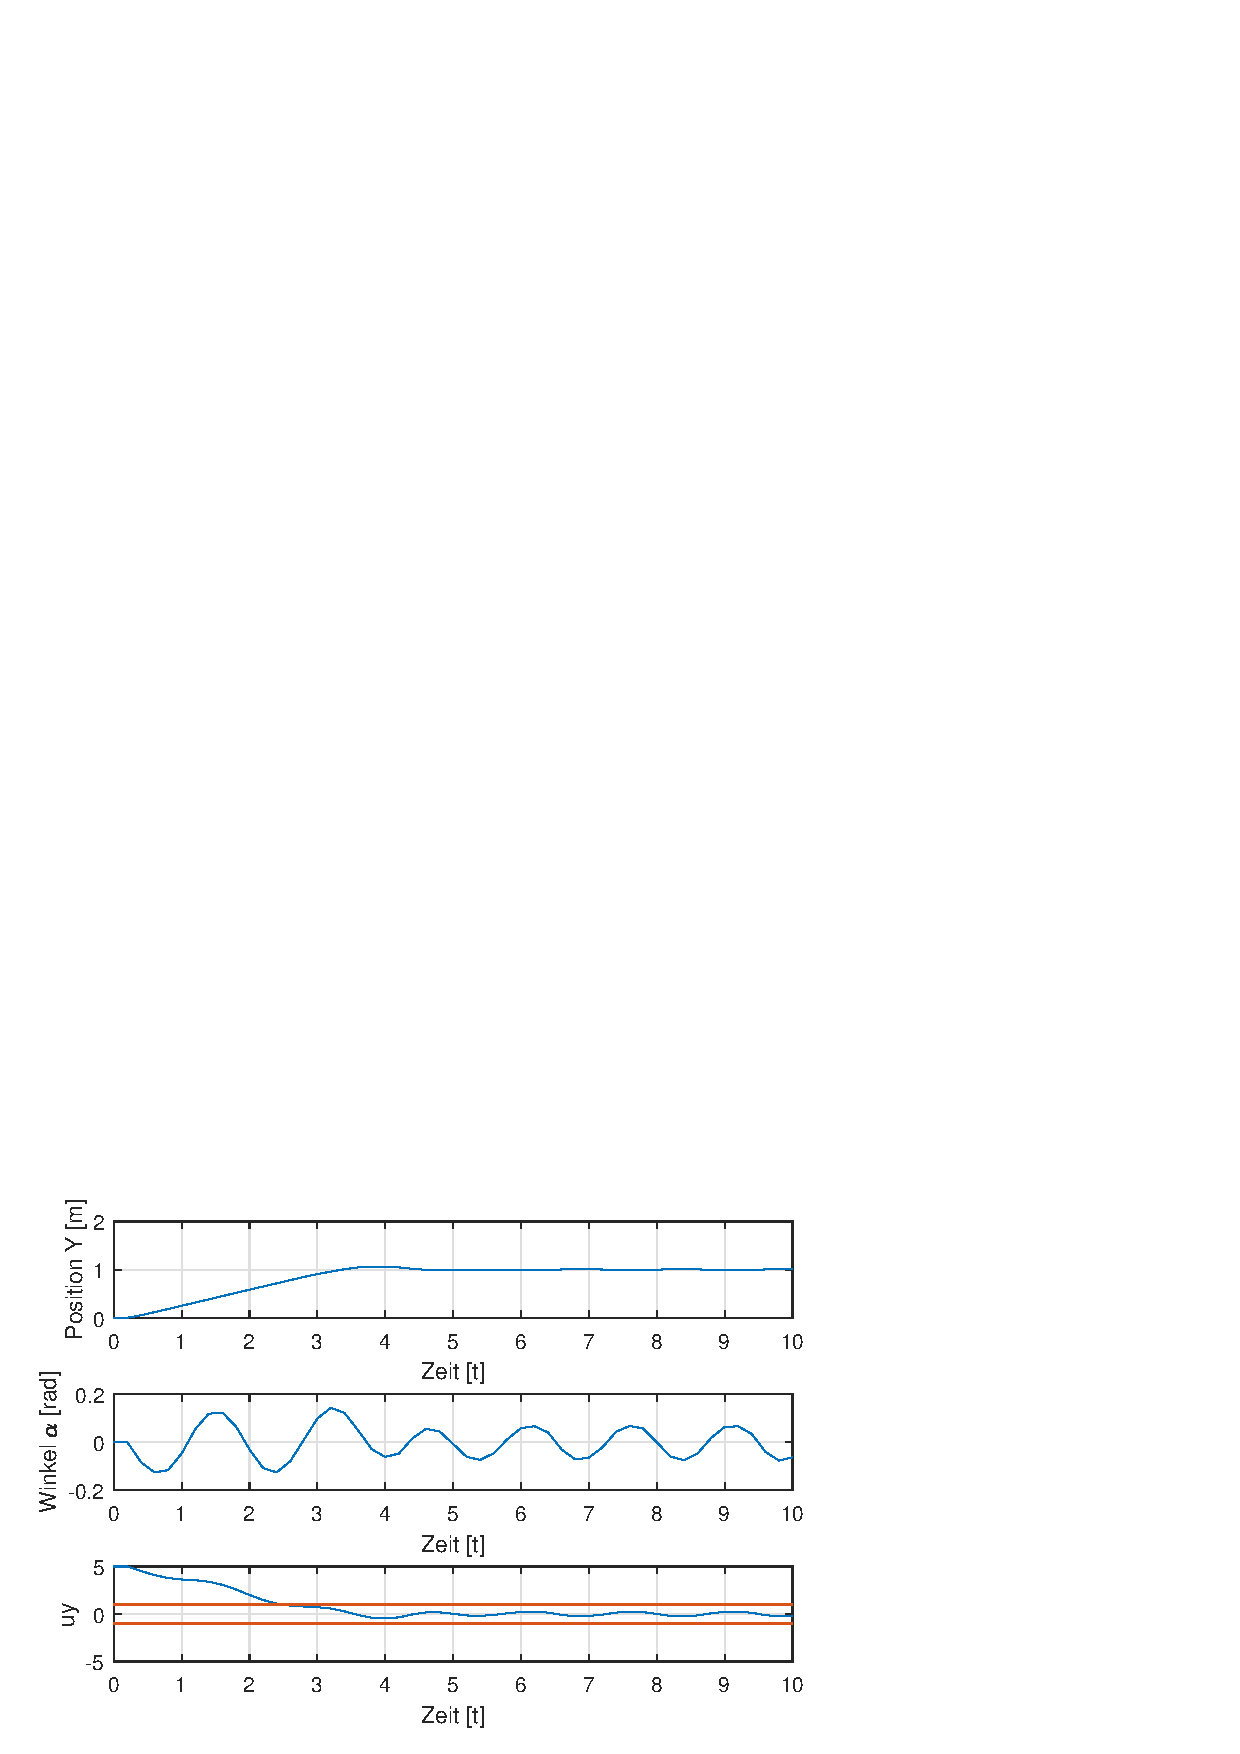
\includegraphics[width=0.6\textwidth]{Figure45a200mT}
	\caption{Verlauf des Experimentes mit einer Abtastzeit von 200ms}
	\label{img:grafik-dummy}
\end{figure}
Beobachtung:
Bei der Abtaszeit im oberen Grenzbereich schaukelt sich die eigentliche Grundbewegung auf und die Pendelbewegung wird eher verstärkt als gedämpft. Das sorgt für ein stärkere Pendelbewegung als die ungeregelte Bewegung. 
\item Die Abtastzeit wird auf t = 1 ms festgelegt.
\begin{figure}[H]
	\centering
	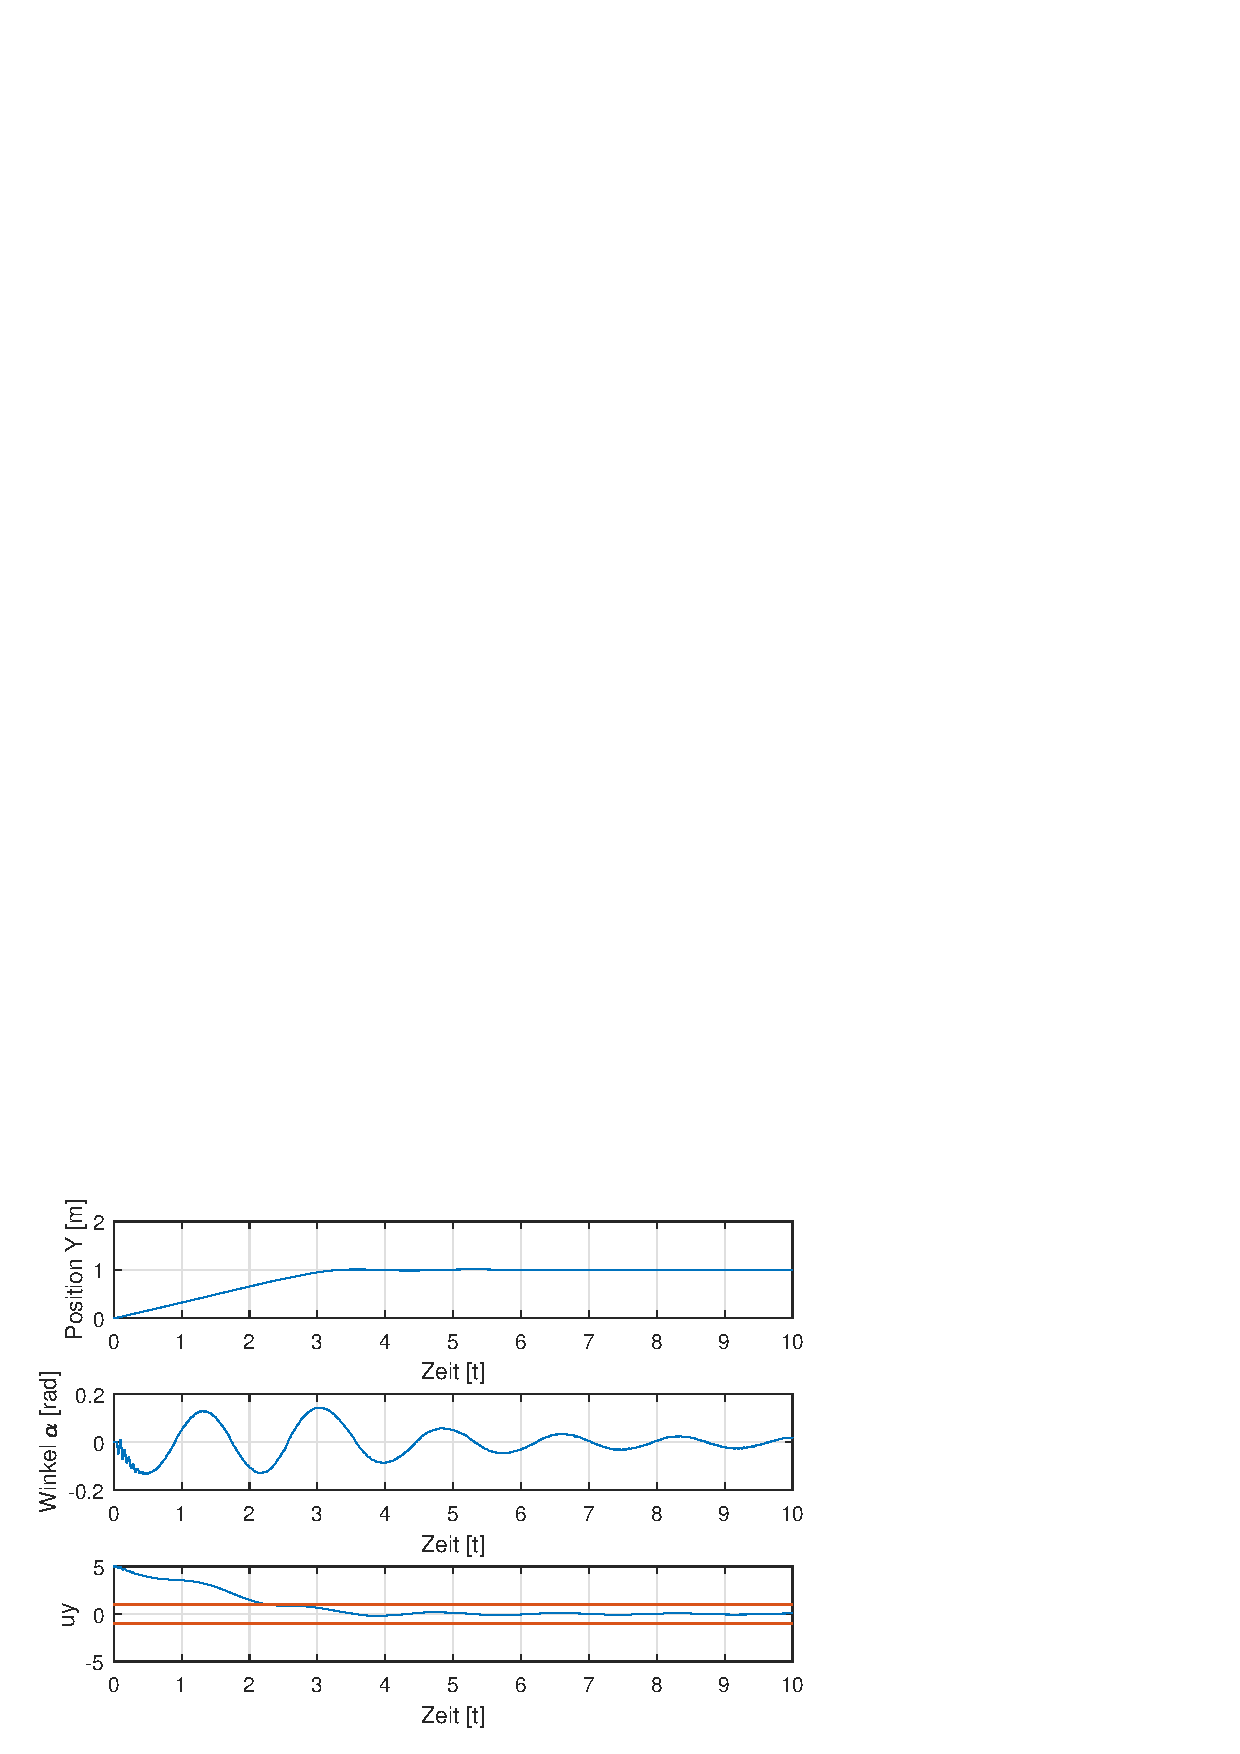
\includegraphics[width=0.6\textwidth]{45a1mT}
	\caption{Verlauf des Experimentes mit einer Abtastzeit von 1ms}
	\label{img:grafik-dummy}
\end{figure}
Beobachtung: 
Bei dieser kleineren Abtastzeit arbeitet der Regler so, dass das Schwingen des Seils stark vermieden wird. Es sorgt dafür, dass das die Auslenkung des Seils verringert wird.
\end{enumerate}
\textbf { Fazit:} Das Fazit, was aus diesem Versuch gezogen werden muss ist, dass die diskretisierung einer Messung und die diskretisierung eines Reglers in ausreichender Genauigkeit vorgenommen werden muss.
\subsubsection{Warum macht eine Erweiterung um einen PD-Regler Sinn?}
\begin{figure}[H]
	\centering
	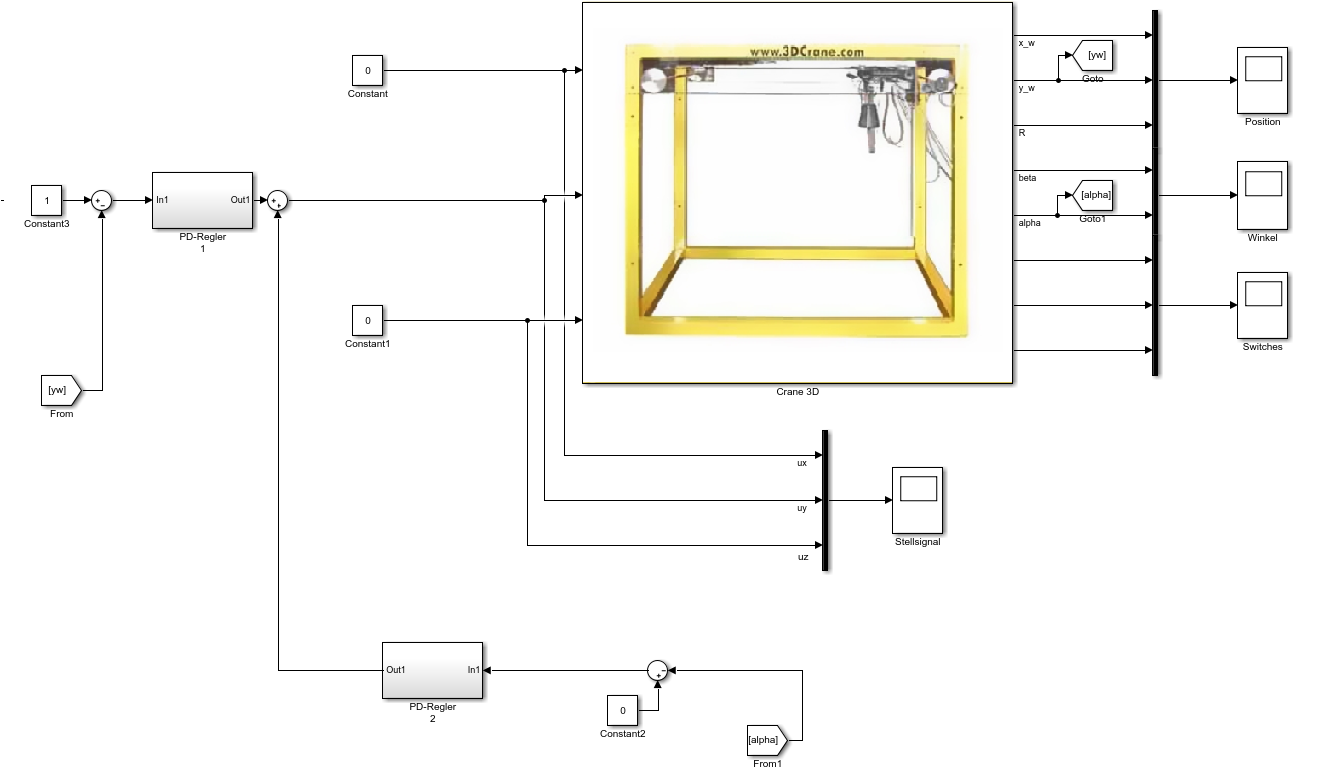
\includegraphics[width=0.6\textwidth]{PDRegler.png}
	\caption{Aufbau der PD-Regelung im realen System}
	\label{img:grafik-dummy}
\end{figure}
Dazu müssen wir uns die Beschreibung des Systems anschauen und mit den Zielen der Regelung vergleich. Es soll die Abweichung des Seilwinkels möglichst gering sein und die Position des Krans möglichst exakt erreicht werden. Da ein P-Regler immer eine dauerhafte Regelabweichung mit sich bringt, so kann mit dem PD-Regler gut auf eine schnelle Änderung reagiert werden, da dieser besser auf die Veränderung einer Regelgröße reagiert. Diese Veränderung kann gut mit einem D-Regler geregelt werden um weiter einer möglichen dauerhaften Abweichung Regelungstechnik zu begegnen werden die P-Regelanteile genutzt. Dies macht den PD-Regler an dieser Stelle zum idealen Regler für den Kran.

\subsubsection{Test des PD-Regler im Realen System}
\begin{figure}[H]
	\centering
	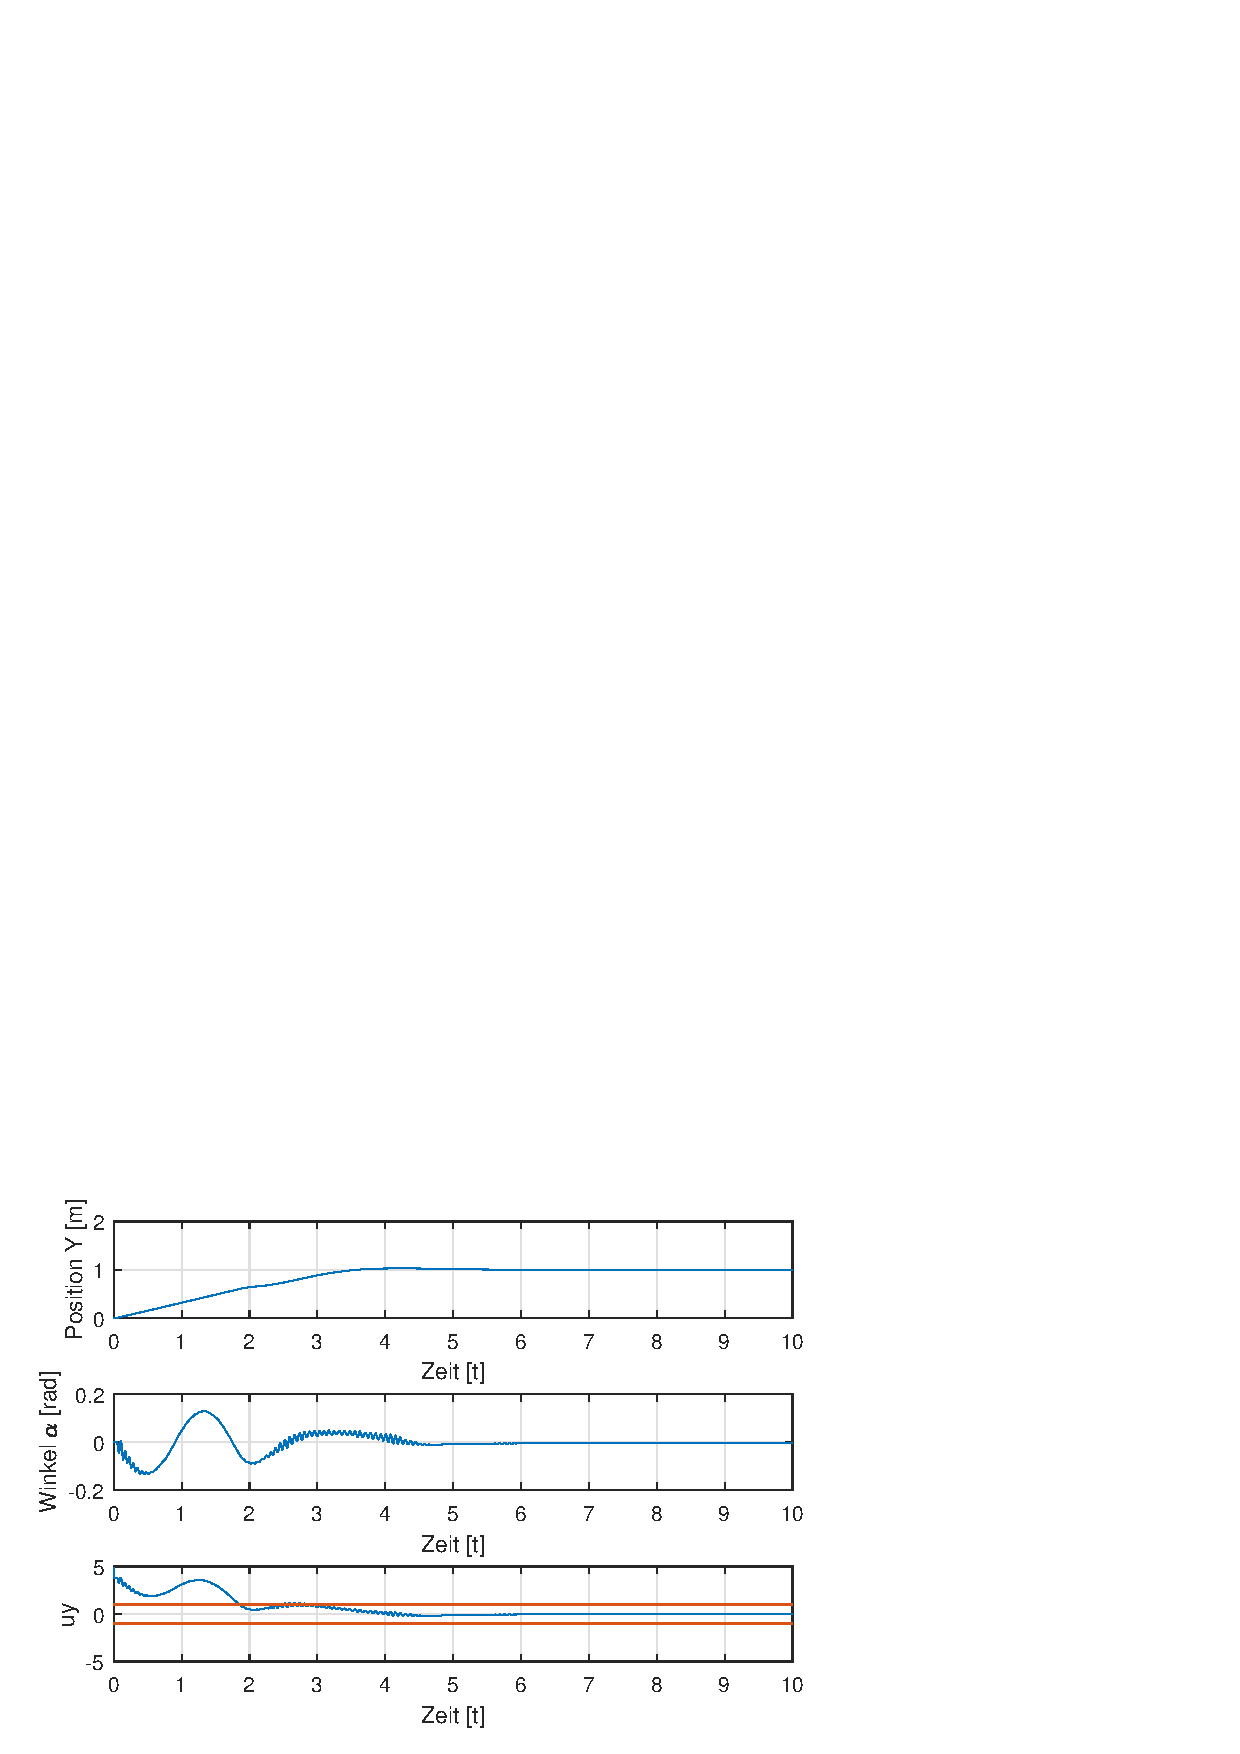
\includegraphics[width=0.6\textwidth]{PD-ReglerTestReal}
	\caption{Aufbau der PD-Regelung im realen System}
	\label{img:grafik-dummy}
\end{figure}
Bei diesem Versuch lässt sich beobachten, dass es in der Eingelphase, wenn die Überlagerung des P-Reglers nicht mehr mehr in der Sättigung des Stellmotors ist, ein zittern der Kurve zu beobachten. Auch beim Versuch im realen System gibt es dieses Regelflackern.

\subsubsection{Filterung über ein PT-1 Glied}
Es soll zu dem Regler ein PT-1 Filter implementiert werden. Die Idee bei diesem Versuch ist es, dass das Rauschen unterdrückt wird und die Zitterbewegungen am Ende zu vermeiden und damit gleichzeitig auch die Ausregelzeit verkürzen. Wir implementieren dazu das PT-1 Glied in das gegebene Simulinkmodell des Vorversuchs. Dieses Modell wird sowohl im Winkel, wie auch in der Streckenregelung im ein PT-1 Glied erweitert.

\begin{figure}[H]
	\centering
	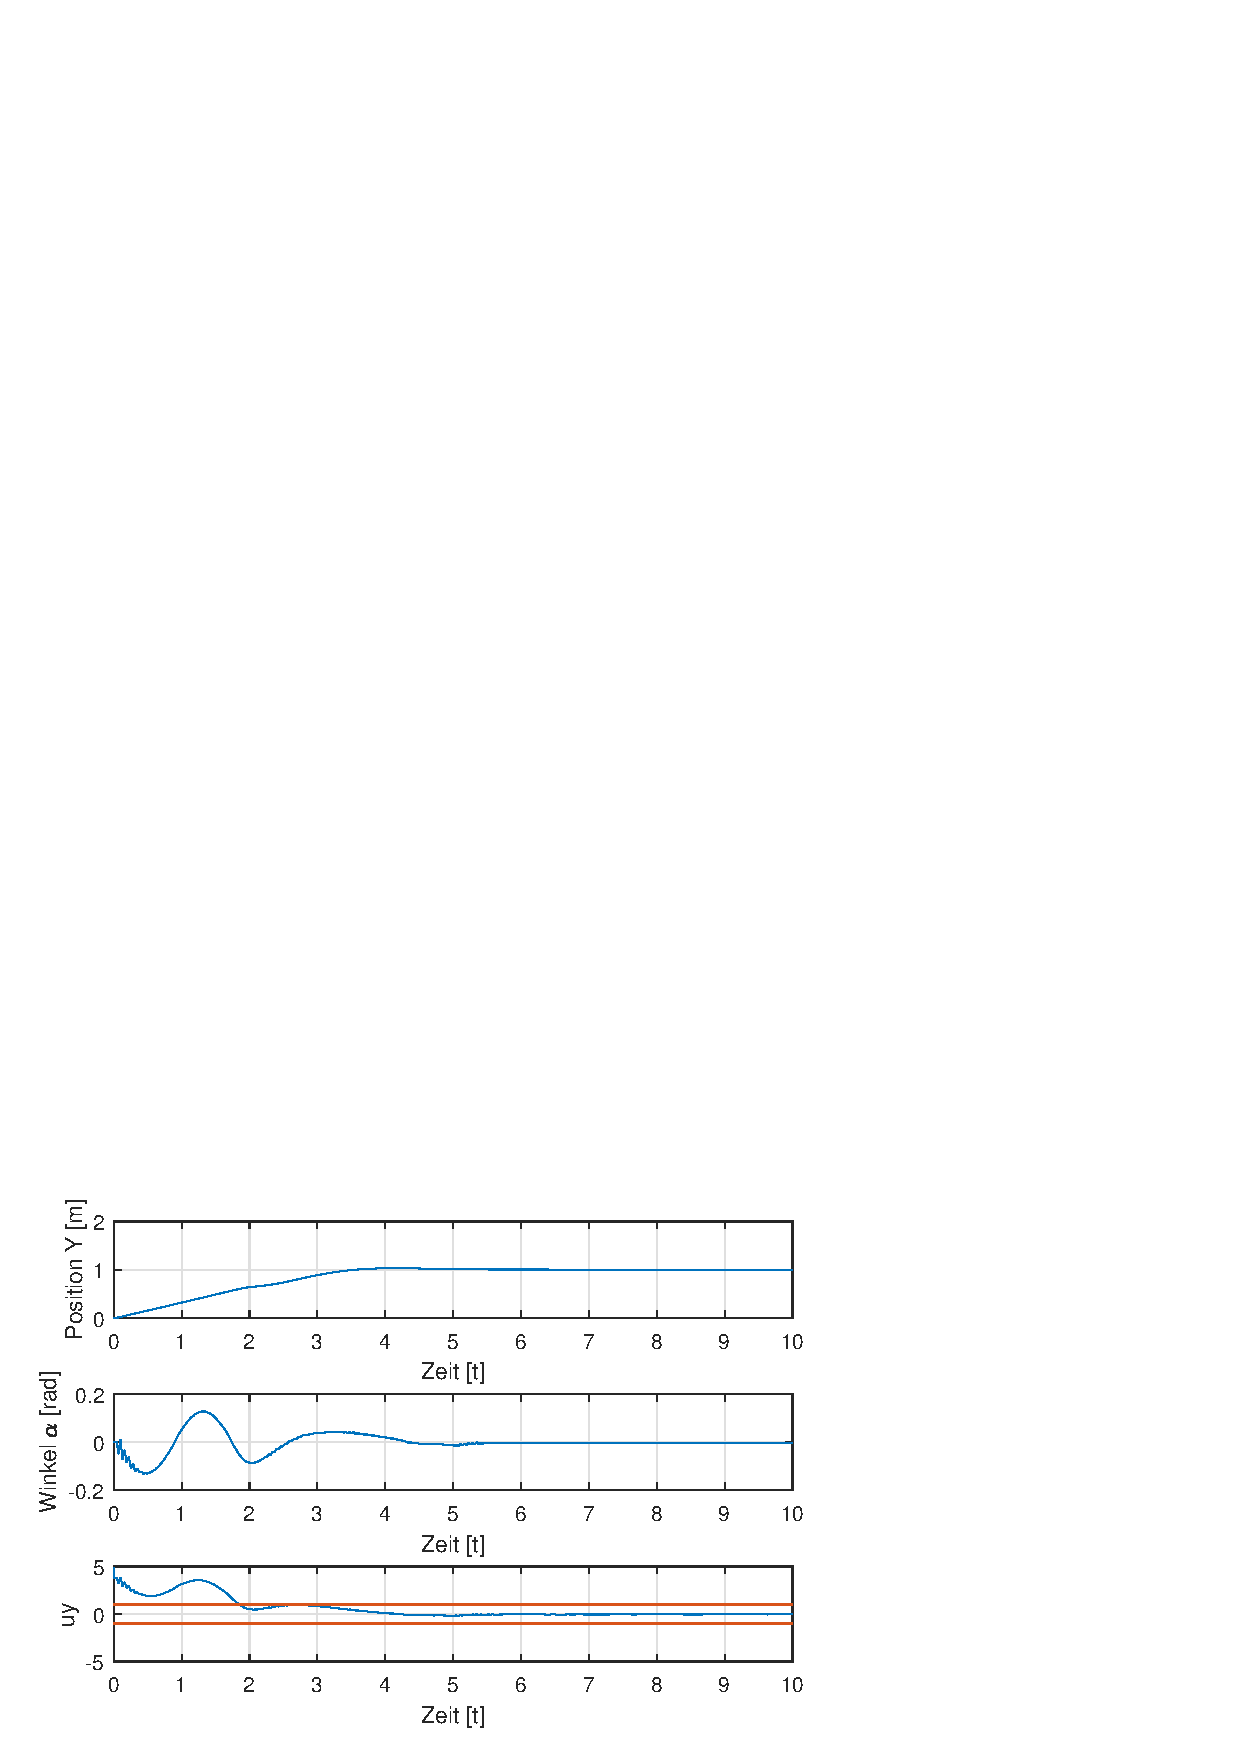
\includegraphics[width=0.6\textwidth]{Figure45b1}
	\caption{Aufbau der PD-Regelung im realen System ergänzt mit einer PT1-Strecke zur Filterung der Kleinstabweichungen}
	\label{img:grafik-dummy}
\end{figure}

\subsection{Regelung mit zusätzlicher Stellgrößenbeschränkung}
\subsubsection{Kann Stellgrößenbeschränkung für eine Regelverbesserung sorgen?}
Die neue Struktur korregiert das Problem in gewisser Weise, weil das Verhältnis von Wegstreckeänderung zu Winkel eingeschränkt werden kann. Wenn der Stellgrößenanteil, der Wegstrecke nicht mehr voll ausgestreckt werden kann, begrenzt sich die Geschwindigkeit mit der der Krankwagen bewegt werden kann. Dieser Regelgrößenanteil steht dann der Regelung des Seilwinkels zu. Zusätzlich ist eine begrenzte Beschleunigung des Kranwagens nicht mehr dazu in der Lage einen unbegrenzt großen Winkel zu produzieren. Daraus lässt sich Schlussfolgern, dass eine Stellgrößenbeschäkung die Regelungsgenaurigkeit verbessert.
\subsection{Testen dieser theoretische Stellgrößenbeschränkung im realen Versuchsaufbau}
Nach einigen Versuchsreihen wurde ein Stellte sich der beste Kompromiss bei einer Stellgrößenbeschränkung auf einen Wert von 0,9 ergeben. Das Ergebnis dieser Dokumentation wurde hier dann festgehalten.

\begin{figure}[H]
	\centering
	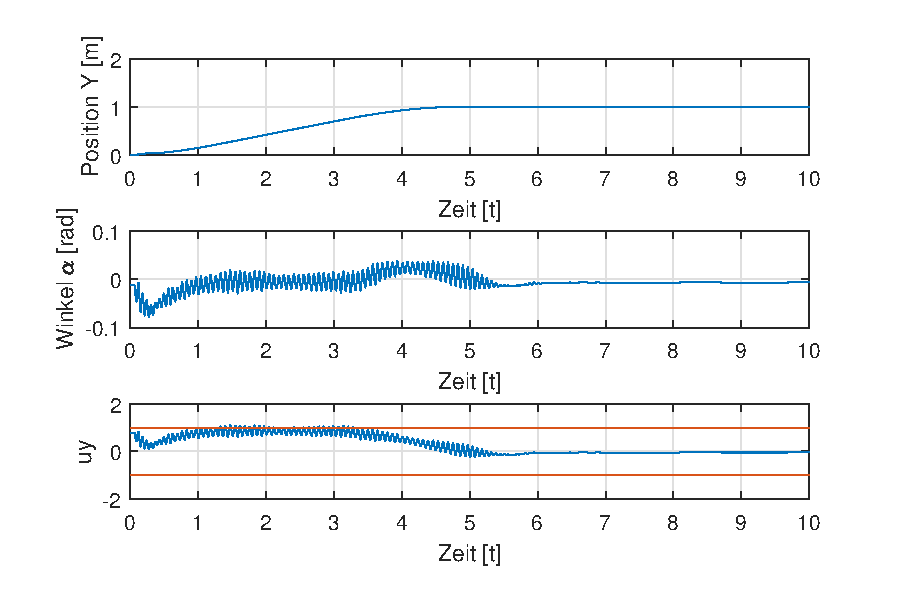
\includegraphics[width=0.6\textwidth]{Figure45b5mitSaturation}
	\caption{Regelungsdarstellung mit der Stellgrößenbeschränkung und einem PD-Regler}
	\label{img:grafik-dummy}
\end{figure}

Es lässt sich dabei festhalten, dass zwar eine Regelverbesserung eintritt, allerdings das Zittern des Versuchs erneut vorhanden ist. Vielleicht könnte dies mit dem im Kapitel vorher gezeigten Filterglied in der Griff verbessert werden. Hierbei muss also die Abtastzeit der Messeinrichtung berücksichtigt werden um dieses Zittern zu vermieden und eine bessere Regelaussteuerung zu ermöglichen.
\subsection{Regelung der x- und y- Achse}

%Modell zum Einfügen eines Bildes
%\begin{figure}[H]
%	\centering
%	\includegraphics[width=0.8\textwidth]{}
%	\caption{Teamlogo: Team A}
%	\label{img:grafik-dummy}
%\end{figure}
\newpage
\listoffigures


\end{document}